%%%%%%%%%%%%%%%%%%%%%%%%%%%%%%%%%%%%%%%%%%%%%%%
%
% Template per Elaborato di Laurea
% DISI - Dipartimento di Ingegneria e Scienza dell’Informazione
%
% update 2015-09-10
%
% Per la generazione corretta del 
% pdflatex nome_file.tex
% bibtex nome_file.aux
% pdflatex nome_file.tex
% pdflatex nome_file.tex
%
%%%%%%%%%%%%%%%%%%%%%%%%%%%%%%%%%%%%%%%%%%%%%%%

% formato FRONTE RETRO
\documentclass[epsfig,a4paper,11pt,titlepage,twoside,openany]{book}
\usepackage{epsfig}
\usepackage{plain}
\usepackage{setspace}
\usepackage{float}
\usepackage[paperheight=29.7cm,paperwidth=21cm,outer=1.5cm,inner=2.5cm,top=2cm,bottom=2cm]{geometry} % per definizione layout
\usepackage{titlesec} % per formato custom dei titoli dei capitoli

%%%%%%%%%%%%%%
% supporto lettere accentate
%
%\usepackage[latin1]{inputenc} % per Windows;
\usepackage[utf8x]{inputenc} % per Linux (richiede il pacchetto unicode);
\usepackage{listings}
\usepackage{color}
\usepackage{graphicx}
\graphicspath{ {images/} }

\definecolor{dkgreen}{rgb}{0,0.6,0}
\definecolor{gray}{rgb}{0.5,0.5,0.5}
\definecolor{mauve}{rgb}{0.58,0,0.82}

\lstset{frame=tb,
  language=Java,
  aboveskip=3mm,
  belowskip=3mm,
  showstringspaces=false,
  columns=flexible,
  basicstyle={\small\ttfamily},
  numbers=none,
  numberstyle=\tiny\color{gray},
  keywordstyle=\color{blue},
  commentstyle=\color{dkgreen},
  stringstyle=\color{mauve},
  breaklines=true,
  breakatwhitespace=true,
  tabsize=3
}
%\usepackage[applemac]{inputenc} % per Mac.

\singlespacing

\usepackage[english]{babel}

\begin{document}

  % nessuna numerazione
  \pagenumbering{gobble} 
  \pagestyle{plain}

\thispagestyle{empty}

\begin{center}
  

  \vspace{2 cm} 
  \Huge\textsc{{University of Trento}\\}
  \vspace{1 cm} 
  \LARGE\textbf{Department of Information Engineering and Computer Science\\}

  \vspace{1 cm} 
   \begin{figure}[h!]
    \centerline{\psfig{file=images/logoUNITN.jpg,width=0.3\textwidth}}
  \end{figure}	
  \vspace{1 cm}
  \Large\textbf{Bachelor’s Degree in Computer Science}

  \vspace{2 cm} 
  \Large\textsc{Final Dissertation\\}
  \vspace{1 cm} 
  \Huge\textbf\textsc{Evaluating MongoDb Performance:\\}
  \LARGE{\bf{\it{How and where NoSQL databases are getting over Relational Databases}}}


  \vspace{2 cm} 
  \begin{tabular*}{\textwidth}{ c @{\extracolsep{\fill}} c }
  \Large{Supervisor} & \Large{Student}\\
  \Large{Alberto Montresor}& \Large{Michele Romani}\\
  \end{tabular*}

  \vspace{2 cm} 

  \Large{Academic year 2015/2016}
  
\end{center}



  \clearpage
 
%%%%%%%%%%%%%%%%%%%%%%%%%%%%%%%%%%%%%%%%%%%%%%%%%%%%%%%%%%%%%%%%%%%%%%%%%%
%%%%%%%%%%%%%%%%%%%%%%%%%%%%%%%%%%%%%%%%%%%%%%%%%%%%%%%%%%%%%%%%%%%%%%%%%%
%% Nota
%%%%%%%%%%%%%%%%%%%%%%%%%%%%%%%%%%%%%%%%%%%%%%%%%%%%%%%%%%%%%%%%%%%%%%%%%%
%% Sezione Ringraziamenti opzionale
%%%%%%%%%%%%%%%%%%%%%%%%%%%%%%%%%%%%%%%%%%%%%%%%%%%%%%%%%%%%%%%%%%%%%%%%%%
%%%%%%%%%%%%%%%%%%%%%%%%%%%%%%%%%%%%%%%%%%%%%%%%%%%%%%%%%%%%%%%%%%%%%%%%%%
  \thispagestyle{empty}

\begin{center}
  {\bf \Huge Acknowledgements}
\end{center}

\vspace{4cm}


\emph{
 In my experience, people that live around us always contribute in some way in what we do. %Unless you are a hermit, of course. 
And there are different kinds of support people can give you, depending on your relation with them. 
On the affective side, I’d like to thank my family for always believing in me and in what I do, and supporting me in my choices.
I thank my girlfriend and my friends for their support and the priceless time I always spend with them. And my course mates, for all the time we studied together sharing knowledge and useful suggestions.
On the professional side, first I’d like to express my gratitude to my Supervisor and Professor Alberto Montresor for the passion he transmitted me during the course of Algorithms, for involving me in interesting projects and for supervisioning me during these last months.
I’d also like to thank my Erasmus Professor Erki Eassar for his skill in making me appreciate the course of Databases and for sharing me useful suggestions and essential material.
At last, I’d like to acknowledge my internship tutors in Tai, Andrea Carpineti and David Votino, for their technical and motivational suggestions about the project \textsc{MongoDB Performance}, and my colleague Bruno Graziano for his help in configuring and maintaining the system of virtual machines that hosted my clients and my Mongo cluster during the main tests. 
Have a good reading.
}


  \clearpage
  \pagestyle{plain} % nessuna intestazione e pie pagina con numero al centro

  
  % inizio numerazione pagine in numeri arabi
  \mainmatter

%%%%%%%%%%%%%%%%%%%%%%%%%%%%%%%%%%%%%%%%%%%%%%%%%%%%%%%%%%%%%%%%%%%%%%%%%%
%%%%%%%%%%%%%%%%%%%%%%%%%%%%%%%%%%%%%%%%%%%%%%%%%%%%%%%%%%%%%%%%%%%%%%%%%%
%% Nota
%%%%%%%%%%%%%%%%%%%%%%%%%%%%%%%%%%%%%%%%%%%%%%%%%%%%%%%%%%%%%%%%%%%%%%%%%%
%% Si ricorda che il numero massimo di facciate e' 30.
%% Nel conteggio delle facciate sono incluse 
%%   indice
%%   sommario
%%   capitoli
%% Dal conteggio delle facciate sono escluse
%%   frontespizio
%%   ringraziamenti
%%   allegati    
%%%%%%%%%%%%%%%%%%%%%%%%%%%%%%%%%%%%%%%%%%%%%%%%%%%%%%%%%%%%%%%%%%%%%%%%%%
%%%%%%%%%%%%%%%%%%%%%%%%%%%%%%%%%%%%%%%%%%%%%%%%%%%%%%%%%%%%%%%%%%%%%%%%%%

    % indice
    \tableofcontents
    \clearpage
    
    
          
    % gruppo per definizone di successione capitoli senza interruzione di pagina
    \begingroup
      % nessuna interruzione di pagina tra capitoli
      % ridefinizione dei comandi di clear page
      \renewcommand{\cleardoublepage}{} 
      \renewcommand{\clearpage}{} 
      % redefinizione del formato del titolo del capitolo
      % da formato
      %   Capitolo X
      %   Titolo capitolo
      % a formato
      %   X   Titolo capitolo
      
      \titleformat{\chapter}
        {\normalfont\Huge\bfseries}{\thechapter}{1em}{}
        
      \titlespacing*{\chapter}{0pt}{0.59in}{0.02in}
      \titlespacing*{\section}{0pt}{0.20in}{0.02in}
      \titlespacing*{\subsection}{0pt}{0.10in}{0.02in}
      
      % sommario
      \chapter*{Summary} % senza numerazione
\label{Summary}

\addcontentsline{toc}{chapter}{Summary} % da aggiungere comunque all'indice

The IT world is evolving faster and faster every year, with new breaking technologies coming to our lives, even changing our way to communicate and live in our society. With the advent of social networks, cloud storage and cloud computing, a new definition for the amount of data they involve has been coined: \textsc{Big Data}\footnote{https://datascience.berkeley.edu/what-is-big-data/}.
The challenge of Big Data involves both developing better retrieving solutions using advanced data mining techniques and functional storage solutions \cite{whitepaper}.
Several companies are switching their old systems and technologies to more scalable and reliable solutions to optimize their costs in terms of time and money, improving their profits.
The company in which I am actually working entrusted me to develop a software in order to evaluate \textsc{MongoDB} \footnote{https://www.mongodb.com/what-is-mongodb}, a new non-relational database technology in anticipation of a new  contract from a customer that needs to support an application with several hundred thousand of users and millions of records.
The challenge was to obtain acceptable results from Mongo in stressing conditions like a production software: retrieving data in less than 2 seconds, preventing loss of data and most importantly, preventing a system crash of the database.
I entirely developed a Java software based on the Spring framework, following my project leader and my tutor directives, with the functionality to launch specific benchmark tests aimed at stress-testing and maybe even crashing a virtual machine running a MongoDB instance.
For my architecture I used the technique of \textsc{Microservices} \footnote{http://microservices.io/patterns/microservices.html}, that consists in building a modular application, with each module dedicated to a specific service. It is an advanced development technique that is getting more and more successful, also thanks to famous use cases such as Netflix, with the strength of easy re usability and maintainability of the software.
My choice of this technique is due to a possible future experimentation of other storage technologies, even relational, as the modularity of the applications allow to quickly develop and connect a new module with drivers for other Database Management Systems.
The choice of MongoDB was made by both our manager and our customer because of its ease of configuration and its availability as 
an open-source software.
This research aims to explain many reasons why NoSQL technologies are taking over the well-known relational databases in new enterprise applications, focusing on selected use cases.
In particular, the committed software had to perform a stress-test on MongoDB to verify if it could stand the customer requirements.
The team involved 3 persons:
\begin{itemize}
  \item me as Software Developer.
  \item an internal System Engineer that helped me configure MongoDB instances on different nodes (depending on the test requirements) and the virtual machines that have been used through the evaluation.
  \item an internal Software Engineer, my stage tutor, that helped me define the architecture of the application and choose the right frameworks for both backend and frontend. He also contributed in defining test cases and testing the features of the software.
\end{itemize}
To clarify, the research does not demonstrate that NoSQL technologies are a better choice than Relational DBMS in any case, nor that the relational databases will get outdated and out of use.
In fact, both of them have strengths and weaknesses based on the situation in which they are used.
The future of databases will likely involve the parallel use of different technologies or maybe a "fusion" like, for example, NewSQL databases that are currently under experimental development.
But even tough relational databases are not going to disappear soon, we will explain why NoSQL are really taking over them in the highly demanding requests of the new market of Big Data challenging applications in terms of high scalability, usability and performance.
This will likely lead to a relegation of Relational DBMS to specific roles in a system or to specific use cases in which they still have better reliability or even better performance than NoSQL regardless their higher cost of configuration and maintainability and their restrictions as explained by the \textit{CAP theorem} \footnote{Also named Brewer's theorem, will be explained in chapter 2}.
\textsc{MongoDb Performance} was developed entirely in Java on the backend side, while the frontend side was developed in HTML 5, CSS and Javascript.
It depends on several frameworks and libraries, among which the most relevant are:
\begin{itemize}
    \item \textit{Java Spring} \footnote{https://spring.io} - The future of Java Development, based on REST calls and Annotations.
    \item \textit{AngularJS} \footnote{https://angularjs.org} - An essential web framework to build single page applications with dynamic loading of contents, used in combination with \textit{Twitter Bootstrap} \footnote{http://getbootstrap.com}.
    \item \textit{MetricsGraphics.js}\footnote{http://www.metricsgraphicsjs.org} - A versatile Javascript framework based on D3, used to plot data.
\end{itemize}
The code of the project can be visualized on GitHub \footnote{https://github.com/BRomans/mongodb-performance-app} only after authorization as its property rights are owned by the company.
\ \clearpage





%%%%%%%%%%%%%%%%%%%%%%%%%%%%%%%%%%%%%%%%%%%%%%%%%%%%%%%%%%%%%%%%%%%%%%%%%%
%%%%%%%%%%%%%%%%%%%%%%%%%%%%%%%%%%%%%%%%%%%%%%%%%%%%%%%%%%%%%%%%%%%%%%%%%%
%% Nota
%%%%%%%%%%%%%%%%%%%%%%%%%%%%%%%%%%%%%%%%%%%%%%%%%%%%%%%%%%%%%%%%%%%%%%%%%%
%% Sommario e' un breve riassunto del lavoro svolto dove si descrive 
%% l’obiettivo, l’oggetto della tesi, le metodologie e 
%% le tecniche usate, i dati elaborati e la spiegazione delle conclusioni 
%% alle quali siete arrivati.
%% Il sommario dell’elaborato consiste al massimo di 3 pagine e deve contenere le seguenti informazioni: 
%%   contesto e motivazioni
%%   breve riassunto del problema affrontato
%%   tecniche utilizzate e/o sviluppate
%%   risultati raggiunti, sottolineando il contributo personale del laureando/a
%%%%%%%%%%%%%%%%%%%%%%%%%%%%%%%%%%%%%%%%%%%%%%%%%%%%%%%%%%%%%%%%%%%%%%%%%%
%%%%%%%%%%%%%%%%%%%%%%%%%%%%%%%%%%%%%%%%%%%%%%%%%%%%%%%%%%%%%%%%%%%%%%%%%%      
      
      %%%%%%%%%%%%%%%%%%%%%%%%%%%%%%%%
      % lista dei capitoli
      %
      % \input oppure \include
      %
      \newpage
      \chapter{Introduction}
\label{cha:intro}

In the first two parts of this chapter a brief overview will explain the most known databases technologies while in the last part NoSQL databases will be introduced through the descrption of the most famous implementations from which many others derive.


\section{Discovery of NoSQL technologies}
\label{sec:context}

Commonly students have their first encounters with database technologies during their studies in high school or bachelor degree and, to better understand all the fundamentals concepts, they are taught the basic principles of relational databases.
It i’s the most common choice of every school teaching the very foundation of Databases to make students understand the the meaning of \textit{CRUD operations, relations, consistency, redundancy} \footnote{https://en.wikipedia.org/wiki/Create,\_read,\_update\_and\_delete}, etc... and how to correctly set up the entities of their systems following proven patterns and constraints.
Detaching from well-known developing habits is not always so simple, but it is necessary to understand why big companies such as Facebook decided to invest money in developing their own database solution, Cassandra, instead of using an existing relational database.
It is important to know that there are many different ways to build a database, some are better than others in certain use cases. Nowadays, an huge amount of data are spread around the world everyday through the Web and it needs to be stored and retriewed quickly to save companies' money and give the users a perfect feeling of responsivity\cite{}.
But let’s start from the beginning to get an overview of a technology we rely on every day, even without being aware of its presence in every single application we use.


\section{Databases}
\label{sec:problem}

A Database is an organized collection of data even though we often use the term to refer to the entire database system. The Database Management System, or DBMS, is the name of the entire system that handles data, transactions, relations and eventually problems.
The term DBMS has been replaced by RDBMS in the common language, that stands for Relational Database Management Systems, since for decades the relational model has been a standard for data storage.


\subsection{Relational Databases}
\label{sec:description}

Probably the most popular and for many years also most used model, a relational database is composed by tables representing entities (users, customers, courses...) where each column represents a field or attribute and each row represents a record.
Tables can have relations each other with the use of foreign keys, and each table has a primary key that is unique on each record.
It’s fundamental for a good design of a relational database that its schema is in \textit{Normal Form}, following three main steps:
\begin{itemize}
	\item \textit{First Normal Form} : Eliminating groups of repeated data and creating a table for each group of related data identified with a primary key.
	\item \textit{Second Normal Form} : Moving all identical set of values for multiple records to a new table and using a foreing key to link them.
	\item \textit{Third Normal Form} : Removing all fields not dependent on the primary key or, if they are necesary, putting them into another table.
\end{itemize}
Apart from Normal Form, to ensure that a relational database guarantees the reliability of its transactions it must ensure ACID\footnote{http://www.service-architecture.com/articles/database/acid\_properties.html} properties:
\begin{itemize}
	\item \textit{Atomicity} : A transaction must be completed in all of its parts or none.
	\item \textit{Consistency} : Transactions preserve the integrity of the database and they do not leave the database in an invalid state after occurring.
	\item \textit{Isolation} : Transactions must be isolated to guarantee that any inconsistency does not affect data of other transactions.
	\item \textit{Duraibility} : Completed transactions make changes that must be durable.
\end{itemize}
The most famous relational databases follow SQL syntax that stands for Structured Query Language and is a standard since 1986.
Among this category, the most famous and used are MySQL, PostgreSQL, Microsoft SQL Service, Oracle Database.
\subsection{Navigational Databases}
The first generation of databases used pointers from one record to another to “navigate” the database and that’s why they were called Navigational databases.
The fundamental problem of this kind of database was that the user needed to know the physical structure of the database to query data from it. The only way to add an extra field was achieved only by rebuilding the storage scheme.
In addition, the absence of a standardisation among vendors made those databases disappear quickly in favour of more functional choices

\subsection{Object-oriented Databases}
In the long story of the database evolution, object-oriented databases helped developing the communication between databases and programming languages, but they failed due to their bounds to a specific programming language. They offered advanced features like inheritance and polymorphism and could support a large number of data types.
What is left of their inheritance in the aftermath is the implementation of drivers and bindings between databases and programming language.
NoSQL technologies are a perfect example of the evolution of the idea of object-oriented databases.

\subsection{NoSQL Databases}
The last generation of databases is called NoSQL because of its detachment from the classic relational model in terms of schema and their use of query languages different  than SQL.
They  aim to great performance and scalability, to support the increasing need of those applications that daily transfers huge amounts of data.
Since the category is itself generic, and new different implementations are release every year, they can be broadly divided in those sub-categories:
\begin{itemize}
	\item \textit{Graph databases} : as foundation of this kind of databases there is the graph theory and the concept of nodes and edges. Each node corresponds to an entity and edges correspond to relations between them. They use an index-free adjacency that grants each element a pointer to its adjacent element and does not require the full indexing of the database.
	\item \textit{Key-value stores} : thanks to simple concepte of a key assigned to each value, similarly to has-tables, the model of those databases usually grants higher performance. It is even possible, depending on the database implementation, that a key could be bound to an entire collection of values.
	\item \textit{Document stores} : this is the family which MongoDB belongs and they work around the concept “Document”. Documents are records and they are stored into tables called collections. Usually collections don’t require the same number of fields, so there could be different versions of the same document inside a collection. A great advantage of this model is the ease of data access and manipulation.
\end{itemize}
The core aspect of their implementation is that they have no predefined schema, in addition most of them does not require their records to have the same number of fields if not enforced,  this feature is called Dynamic Schema \footnote{http://blog.rdx.com/is-nosql-the-natural-progression-of-database-technology-0}.
They support to replication of the primary server on many other servers, like MongoDB’s ReplicaSet, and this provides reliability in case of failover of one of the nodes granting no data loss in production applications. Servers execute same transactions and keep their data synchronized to eliminate any errors, and they usually write a backup copy or a snapshot of the data after any operation. As is it possible to imagine, this multi-node architecture cannot fully guarantee the respect of ACID properties and might sometimes present synchronization issues with the possible result of a secondary node becoming primary with partially outdated data.
The absence of constraints on the schema allows query to be executed faster without the need of expensive \textit{join} operations on the collections, but when it comes to execute complex queries NoSQL databases performance fall if they are not well configured.
It is then important to provide a good configuration of the architecture in order make the most of the strengths of those databases.




\subsection{The CAP Theorem}
This theorem, also named Brewer's theorem after the first computer scientist that stated it, states that a distributed computer system cannot simoultaneously provide more than two of the following guarantess: \textit{Consistency\footnote {Every read receives the most recent write or an error}, Availability \footnote{Every requests receives a response, but with no guarantes that it contain the most recent write}, Partition tolerance \footnote{The systems keeps operating despite the delay (or drop) of an arbitrary number of messages }}.
RDBMS for examples, designed with traditional ACID guarantees, choose Consistency and Availability and this is why they have a weak Partition tolerance.
NoSQL databases on the other side are divided in those who prefer Consistency and Partition Tolerance and those who choose Partition Tolerance and Availability.
\begin{figure}[H]
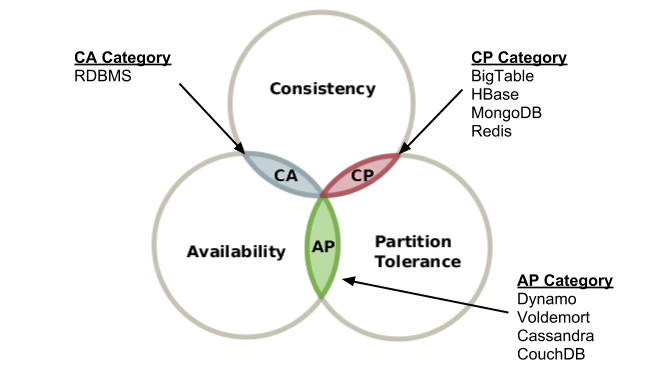
\includegraphics[scale=0.5]{cap-theorem.png}
\centering
\caption{Some famous databases partitoned following the CAP theorem.}
\end{figure}



\section {NoSQL: a brief panoramic over the actual situation}
NoSQL databases area literally spreading around, with many companies and insitutes implementing their own custom version so it would be impossible to describe them all. 
Most of them are new implementations of the pioneers who brought this innovating technology to the market less than 10 years ago, that are briefly described in the following part.

\subsection{MongoDB}
\textsc{MongoDB} is a document-oriented DBMS that uses a JSON-style documents called BSON, making data integration from certain kind of applications easier and faster.
Originally developed as a component of a bigger software, it then became open source in 2009 under the supervision of MongoDB Inc. company.
It offers support for many programming languages such as Java, C++, Python and many others and it’s being used as backed from a large number of web sites and services like eBay, Foursquare, NYTimes among the others.
As db-engines.com reports, it is the most popular NoSQL database now.


\subsection{Google Big Table}
\textsc{Big Table} is the proprietary database system of Google, developed back in 2004 and build on Google File System \footnote{https://en.wikipedia.org/wiki/Google\_File\_System}. It shares the characteristics both of row-oriented databases and column-oriented databases. Google decided to develop its own database with the purpose of scalability and better control over performance: in fact it’s designed to support a data-load of petabytes over thousands of machines.
Big Table supports many Google applications such as Reader, Maps, Books, Earth, Gmail and even YouTube.
Google announced a new version called \textsc{Google Cloud Bigtable }\footnote{https://cloud.google.com/bigtable}, actually in beta, that will be distributed as public version of Big Table.

\subsection{Apache Cassandra}
Another open-source project is \textsc{Apache Cassandra} \footnote{http://cassandra.apache.org}, developed at Facebook in 2007 to improve the research of the internal mail system and then entered in the Incubator project from Apache in 2008 where it begun its growth as DBMS.
Like Big Tables it offers a key-value storage structure with eventual consistency. Each keys correspond to a value and all the values are grouped in families of columns. Families are defined when the database is created and Cassandra adopts an hybrid approach between DBMS oriented to columns and memorization oriented to rows.
Other famous sites than Facebook that uses Cassandra are Twitter and Digg, and many benchmark tests, in terms of performance and scalability confirms Cassandra as the best NoSQL database in the current scenario.

\subsection{Amazon DynamoDB}
\textit{Amazon DynamoDB} \footnote{https://aws.amazon.com/it/dynamodb} is the proprietary database system of Amazon available for developers since 2012, build on the model of Dynamo but with a different implementation and offered as a part of the Amazon Web Services \footnote{https://aws.amazon.com/it} portfolio. The particularity is that DynamoDB allows developer to purchase a service based on the desired throughput rather than the storage, that will be increased by the administrators of the system if needed.
Many programming languages have a DynamoDB binding, including Java, Node.js, Python, Perl and C\#.
Most of the Amazon services uses DynamoDB as storage system.



      \newpage
      \chapter{The Choice}
\label{cha:2}
In this chapter we explain the motivations that determined  MongoDB as choice for the evaluation and consequently the commission among other NoSQL possibilites.
Following there is a deep description of many Mongo core features mostly taken from the official documentation, that could be a good introduction for interested users.

\section{MongoDB}
\label{sec:1}
In evaluating which NoSQL technology could be the best for our company we aimed for a combination between the best performance,  ease of use and understandability of the product as we had no real expert in this field.
This is probably the main reason that made us put Cassandra as secondary makeshift in the evaluation.
Thanks to his functionalities Mongo was the first choice for evaluation: its JSON-like format for data called BSON \footnote{See section 2.2.1} and the simple configuration of its nodes made him the perfect candidate.
Many built-in functions of Mongo automatize the setup of a server and the creation of collections, for example if you try to \textit{insert} a document inside an undefined collection \textit{foo}, Mongo will automatically create this new collection called \textit{foo}.
If you connect to a new database in a Mongo instance and start inserting data, it will automatically create the schema, the collections and give a unique\textit{\_id} to each one of them  with no need of manual interaction from the developer.
MongoDB derives its name from \textit{“humungous”} which means enormous and it fits the idea of application that it was designed to support.
Its data records (or rows) are called \textit{documents} and are stored in tables called \textit{collections}. So when you insert something into a Mongo database you are adding document X to collection Y.
A collection does not require the same schema for all its documents, some of them can have more or less fields than others, but in case of need it is possible to enforce document validation rules in order to accept only documents with the desired schema.

\section{Key features of Mongo}
\label{sec:2}
In this section we introduce all the main features offered by Mongo by default, with a broad overview on them. 
Then we analyze more deeply how Mongo implements those features giving some examples of their usage.

\subsection{BSON data object}
As explained before Mongo uses the BSON \footnote{Binary JavaScript Object Notation - http://bsonspec.org/} documents that are a binary representation for JSON documents, but with more data types.
The\textit{\_id} field is reserved to be used as a primary key and its value must be unique in the collection and of any type other than array.
There are other restrictions on field names: field names cannot start with the dollar “\$” character and not even with the dot “.” character because Mongo uses \textit{dot notation} to access elements of an array or to access the fields of embedded documents.
There is a maximum size for BSON documents of 16 Megabytes. This is to ensure that a single document does not use an excessive amount of RAM, since Mongo uses mostly RAM during its execution, or bandwidth while sending data.
\newpage
There is of course the possibility to store bigger documents with \textit{GridFS API} \footnote{https://www.compose.com/articles/gridfs-and-mongodb-pros-and-cons} provided by Mongo developer team, but it the case of our evaluation it was not needed as we used a relatively small schema for our default document “Fattura”, shown in the previous example, that is a simplification of the billing documents used in our customer’s software.
Here an example of how a BSON Mongo document looks like, based on the model used in our tests:
\begin{lstlisting}
{
        "_id" : ObjectId("588cc30072dd84338cbdec77"),
        "_class" : "it.tai.domain.Fattura",
        "rIndex" : NumberLong(2264826),
        "firstName" : "Michele",
        "lastName" : "Romani",
        "company" : "Tai Software Solutions",
        "taxCode" : "01020304569",
        "vatCode" : "RMNMHL93R28A470U",
        "address" : "Via Monviso 16",
        "municipality" : "Asola",
        "province" : "MN",
        "phone" : "+39 333 3117688",
        "zipCode" : "46041",
        "birthday" : "28-10-1993",
        "username" : "mromani",
        "password" : "ypaLLdNYSOKvaBQNreWyUvGp",
        "email" : "mromani@tai.it"
}
\end{lstlisting}

\subsection{Rich Query Language and CRUD operations}
Mongo provides its own query language that, like the majority of NoSQL databases, is not based on SQL. All its CRUD operations (Create, Read, Update, Delete) are \textit{atomic} on the level of a single document and target a single collection.
For Create operations Mongo uses the following methods:
\begin{itemize}
	\item \textit{Db.collection.insert( )}
	\item \textit{Db.collection.insertOne( )}
	\item \textit{Db.collection.insertMany( )}
\end{itemize}
And their names easily explain their function.
For Read operations Mongo uses the method \textit{db.collection.find( )} in which is possible to specify query filters or criteria using defined operators such as \textit{\$aggregation, \$min, \$max, \$gt, \$lt} and many others that is possible to find in Mongo official documentation.
For Update operations Mongo can identify which documents to update using same syntax as read operations. Those methods then perform the update:
\begin{itemize}
	\item \textit{Db.collection.update( )}
	\item \textit{Db.collection.updateOne( )}
	\item \textit{Db.collection.updateMany( )}
	\item \textit{Db.collection.replaceOne( )}
\end{itemize}
Like Create operations, those methods explain themselves with their name. The upsert operation is performed by specifying its parameter as true.
At last, Delete operations uses the same criteria as Read and Update operations with the following methods:
\begin{itemize}
	\item \textit{Db.collection.remove( )}
	\item \textit{Db.collection.deleteOne( )}
	\item \textit{Db.collection.deleteMany( )}
\end{itemize}

It is very simple to create query data using those methods as they only need some parameters to work. The more basic usage just needs the \textit{\_id} of the target document as only parameter to work.
This is an example of a query that uses an operator to perform a simple research:
\begin{lstlisting}
/* Query on a collection named 'school' to select students between letter M and Z */
db.school.find({
	students: {
		$in: [ "M", "Z"]
	}
});

/* Translated in SQL language */

SELECT * FROM school WHERE students in ("M", "Z");
\end{lstlisting}

Each parameter in a Mongo method is wrapped between {} braces and more parameters can be nested with inner {} braces. 
This is basically how Mongo performs CRUD operations on data. For more examples on how querying embedded documents or arrays it is possible to consult Mongo documentation for further examples.

\subsection {Availability and scalability}
In Mongo, it is possible to obtain high availability thanks to \textit{Replica Set} \footnote{See section 2.6}, a replication facility that provides \textit{automatic failover} and \textit{data redundancy}. In substance, it is a set of Mongo servers (or nodes) that store the same data set, increasing data availability.
For horizontal scalability instead, Mongo’s core functionality is \textit{Sharding} \footnote{See section 2.7}, a facility that distributes data across a cluster of machine using a \textit{Shard Key} to balance data. In latest versions, it is even possible to create zones of data that use the \textit{Shard Key} to direct Mongo operations, covered by a particular zone, only to the shards inside that zone.

\section{Indexes}
\label{sec:3}
Indexes are a special data structure used to store a specific field or set, ordered by its value and they are fundamental for Mongo to perform at its best. This allow to support efficient equality matches and range-based query operations and they can be easily used to sort results with low computational cost.
Every collection has an unique default index \textit{\_id}, created during the creation of the collection and, if not specified in other ways, calculated on the timestamp of the operative system. It is the primary key of the collection and it prevents clients from inserting duplicates, consequently it cannot be dropped. 
In sharded clusters \textit{\_id} is usually used as default \textit{Shard Key} \footnote{See section 2.7.2}, if another field is specified then it must be enforced to be unique.
Indexes typologies are:
\begin{itemize}
	\item \textit{Single Field Index} : classic index on a single field, it can be traversed in both directions for sorting.
	\item \textit{Compound Index} : index on multiple fields, during creation the sorting order must be specified for each field, having 1 for ascending order and  -1 for descending, then they are sequentially applied.
	\item \textit{Multikey Index} : when a compound index holds an array value then it becomes a multikey index having a different key on each element of the array for many combination with other fields within the index. It is not possible to have more than an array field in an index of this type.
	\item \textit{Geospatial Index} : index that is used for geospatial coordinate data, they can be 2d indexes for planar geography or 2dsphere for spherical geometry.
	\item \textit{Text Index} : an index that supports searching for string content, but it can only store ‘root’ words, for example it cannot store prepositions like “the”, “a”, “or” etc.
	\item \textit{Hashed Index} : this index is used to support has based sharding so it indexes the hash of the value of a field. It can be used only for equality matches and cannot support range-based queries.
\end{itemize}
\textit{Hashed Indexes} are very important for Mongo scalability on multiple nodes 
and they have been used in the evaluation to support all tests with a multi node database. They use a hashing function that collapses embedded documents and then computes the hash for the entire value.
Since Mongo automatically computes the hashes when resolving queries, user applications do not need to compute them obtaining higher performance

\section{Storage Engines}
\label{sec:4}
A storage engine is the component of a database managment system responsible of data storaging on disk or in memory. Mongo supports 3 storage engines with different performance depending on specific workloads:
\begin{itemize}
	\item \textit{Wired Tiger} - It is now the default storage engine and provides a document-level concurrency model, also called \textit{checkpointing} and a data compression function that minimizes storage use at the cost of additional CPU.
\textit{Checkpoints} are snapshot of the data saved automatically by Mongo every 60 seconds or after 2 gigabytes of journal data. Thanks to \textit{Wired Tiger}, Mongo can recover data from last checkpoint event without \textit{journaling} data, but wil lose of course any data written after last checkpoint.
\textit{Journal} is a write-ahead transaction log that persists all data modifications between checkpoints and in \textit{Wired Tiger} is active by default, allowing complete data recovery togheter with \textit{checkpoints}.
By default Wired Tiger internal cache uses 50\% of available RAM - 1 GB or 256 MB.
	\item \textit{MMAPv1} - It is  the original storage engine of Mongo and it is still a good choice for worloads with high volume of operations (inserts, reads, updates). It is based on memory mapped files and, like \textit{Wired Tiger}, it uses \textit{Journal} to ensure that every modification  to Mongo data sets are durably written on disk.
With\textit{MMAPv1} Mongo uses the power of 2 sizes allocation so each file has a size that is a power of 2 (32, 64, 128...). The advantages of this strategy are in reducing fragmentation thanks to efficient reuse of freed records and reducing moves thanks to the added padding space given to documents allowing them to grow without requiring a move.
	\item \textit{In-Memory Storage Engine} - 
\end{itemize}


\section{Security}
\label{sec:5}


\section{High Availability}
\label{sec:6}

\subsection{Replica Set and Server Selection Algorithm}

\subsection{Automatic failover and data redundancy}


\section{Horizontal Scalability}
\label{sec:7}

\subsection{Nodes}

\subsection{Shard Keys}

\subsection{Hashed Sharding}

\subsection{Ranged Sharding}

\subsection{Zones}


\section{Some use cases}
\label{sec:8}





      \newpage
      \chapter{The project: MongoDB Performance}
\label{cha:3}
In this chapter the real core of this research, the project \textsc{MongoDB Performance}, is presented starting with the analysis  that we made before developing the software that consequently decreed the implementation choices.
Following there is an overview on the frameworks used and in the end the whole application is described in depth also showing screenshots of the user interface.

\section{Aim of the project and beginning idea}
\label{sec:1}
When benchmarking a product, the standard procedure is to compare it with its competitors, but in this case it took a while to the company to decide which kind of analysis could better fit the availability of time and money.
The beginning idea was in fact to build a software able to perform a stress test on different database technologies, and then to compare those tests and choose the one who could best support the requirements.
Technologies taken in account where MongoDB, Apache Cassandra and PostgreSQL with JSON datatype \footnote{https://www.postgresql.org/docs/9.6/static/datatype-json.html}, but after a meeting with the customer we decided to choose one technology for a specific test using as measurement parameters many benchmarks found on the web and the declared specifications, ease of use and configuration.
PostgreSQL was discarded almost immediately due to lower performance confirmed by third part benchmarks, so MongoDB became the first choice thanks to its simplicity and Cassandra was left as second choice in case Mongo couldn’t satisfy the requirements, even if it seemed to have better results on most of the benchmarks found on the Web. 
As mentioned, the customer gave us specific necessities:
\begin{itemize}
	\item The software counts many hundred thousand active users with thousands of records each one, so the database should be able to support several millions of total records.
	\item It works as a web application and needs to be responsive to give the user the best usage experience, consequently it should query results in no more than 2 seconds.
	\item It contains important billing information, so data cannot be lost.
	\item The web application is online 24/7 and it can be stopped only when releasing a new version. So even in the time slots with more expected traffic, any system crash must be prevented.
\end{itemize}
The final aim of the project so is not a benchmark between different DMBS, but a specific one performed on the chosen technology with the possibility to be eventually extended to other solutions.


\section{Implementation choices and architecture}
\label{sec:2}
It became clear that the beginning idea of a complete benchmark over the most used DBMS was impossible in term of time and money costs.
I decided to develop a modular application following the patterns of microservices. Due to this choice, the final result allows reusing a good part of the software  adding a new module for each eventual DMBS, using the existing code from the MongoDB module and adapting it to another database technology with the proper drivers provided by Java Spring.
In the end thanks to the satisfactory results obtained by MongoDB, there was no need to include other technologies in the benchmark.
The architecture, drew with \textit{Draw.io} \footnote{https://www.draw.io}, presents  both the implemented modules and the possible or discarded modules (dot-line) to give an overview of how a microservices production application should look.
Due to time issues, we decide to not implemented all unnecessary modules like for example the \textit{Authentication Module}.
\begin{figure}
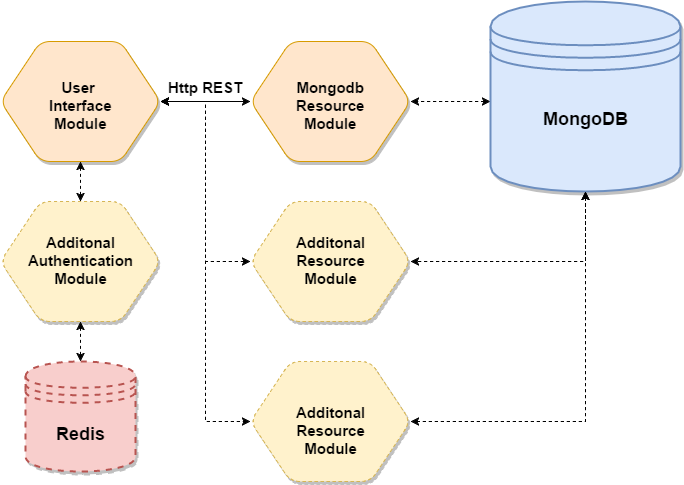
\includegraphics[scale=0.5]{app-architecture.png}
\centering
\caption{Representation of the architecture including possible future implementations}
\end{figure}



\section{Java Spring and AngularJS}
\label{sec:3}
\textsc{Spring} framework has become over the years one of the most popular Java frameworks for building  Enterprise applications, becoming an alternative (or replacement) for the more classical Enterprise Java Beans (EJB)  \footnote{https://en.wikipedia.org/wiki/Enterprise\_JavaBeans}. It introduced the concept of \textit{aspect-oriented} programming that is a programming paradigm that aims to increase modularity by allowing the separation of cross-cutting concerns. It’s composed by many modules, including Spring Security for authorization and authentication, Spring Web for customization of web applications using RESTful web services and Spring Data Access working with \textsc{JDBC} \footnote{http://www.oracle.com/technetwork/java/javase/jdbc/index.html} and object-relational mapping tools to support both relational and NoSQL databases. 
Spring can create standalone “runnable” production-grade applications with Spring Boot, including an embedded Tomcat, and opinionated \textit{POMs} \footnote{https://maven.apache.org/guides/introduction/introduction-to-the-pom.html} to simplify Maven configuration and production-ready features.
Those features, such as metrics, health check together with externalized configuration make it the definitive framework for Java Web applications among the java developer community and  it immediately became my unquestionable choice thanks to its affinity to micro-services model.
On the front-end side, AngularJS was the perfect choice thanks to its natural affinity with Spring and Twitter Bootstrap and its routing management system for dynamic loading dynamic content inside single-page applications. I’ve chosen version 1.6 instead of the new version AngularJS 2, that has a different and more complex implementation and usage based on TypeScript, and I’ve made a wide use of it especially in the User Interface Module that manages the launch and data plotting  of the stress-test.

\section{Microservices and modularity}
\label{sec:4}
The \textit{Microservices Architecture} \footnote{http://microservices.io/patterns} is a modern type of architecture for servers-side enterprise applications. It is designed following specific patterns to support different clients including browsers (desktop or mobile) and native mobile applications. Part of the modules in a Microservices application might expose API to communicate via web services like REST calls, to exchange messages that return HTML/JSON/XML response.
This approach allows major modularity in the developing process of a project involving a team or more where each member (or each team) works only on an assigned module.
The application must be easy to understand in all of its single parts to sustain several deployments on different machines in order to satisfy scalability and availability requirements.
Different frameworks can be used separately on selected modules and functions of the software should not be replicated within the modules.
This type of architecture has many advantages:
\begin{itemize}
	\item Each microservice is a small and independent software, easy to understand and to debug, that in case of fault will not affect other modules \footnote{But its missing functionality could interrupt the application working process.}.
	\item Development is easy to scale, simply connecting a new independent module or machine. In this way each service can be developed and deployed independently.
	\item Eliminates any commitment to a technology stack, in fact if a service needs major changes  it can be rewritten with a new technology stack without interfering with the system.
\end{itemize}
Of course there are some disadvantages to deal with, if an application is developed following Microservices patterns; for example, the additional complexity that a distributed system has with respect to a monolithic system.
A good organization is necessary to manage testing and deployment phases  to keep a low operational complexity in production because the functionality of each single module does not guarantee the functionality of the entire system.
Another problem could be the network overhead generated by several distributed JVM that consume more memory and  network bandwidth than a single monolithic application.
In conclusion, this architecture is highly suggested in those use cases where a distributed system  includes several features (or services) and serves different typologies of clients \footnote{Different apps on different operative systems}, such as Netflix, Amazon and Ebay that switched from a monolithic architecture to microservices.
\begin{figure}[H]
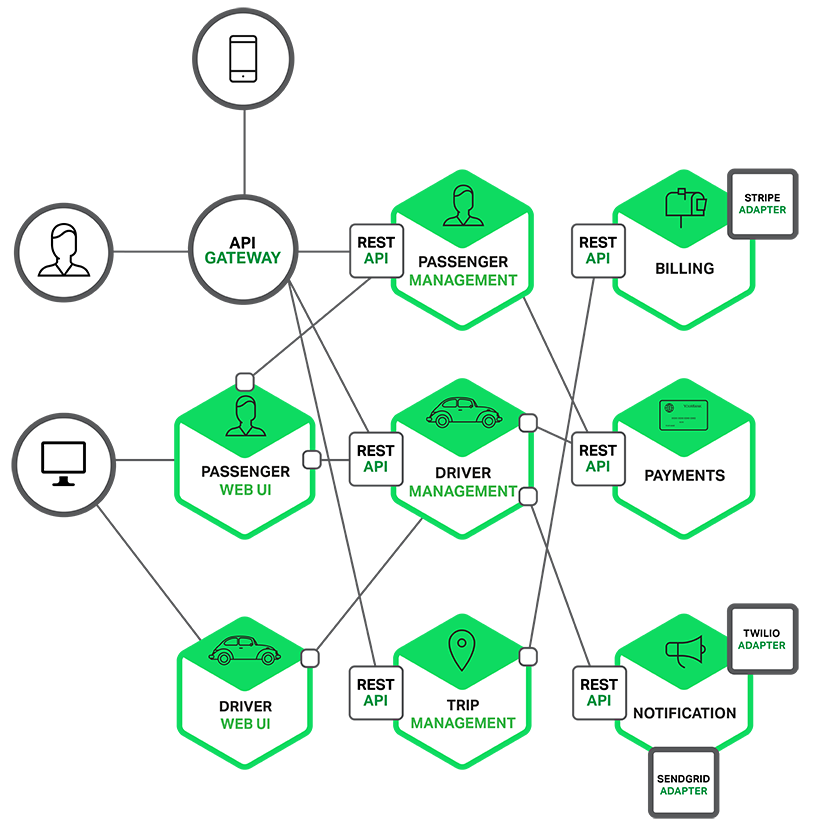
\includegraphics[scale=1.5]{microservices.png}
\centering
\caption{Example of architecture for an application like Uber.} 
\source{https://www.nginx.com/blog/introduction-to-microservices}
\end{figure}

\section{Final modules and possible implementations}
\label{sec:5}

\subsection{Architecture of the application}
The architecture was designed to be reusable and extensible following the theory of microservices. That’s why it was way more complex than the final result, with more modules each dedicated to provide a single functionality. The first design provided the following modules:
\begin{itemize}
	\item \textit{User Interface Module} : it has been kept in the final application and its functionality is related to serve the web resources that compose the front end of the application
	\item \textit{Authentication Module} : it was in beginning implemented and then removed because of possible usage complexity and also because of no real use during the main test. This module was connected to a \textsc{Redis} \footnote{https://redis.io} instance, that is a NoSQL database of key-value type with semi-persistence of the data through snapshots and was used to store the tokens to authenticate users of the application. Since there was need for only one user (me, as admin), the authentication service has been rewritten as angular module \textit{auth.js} for a single user inside the \textit{User Interface Module}. Anyway, it is still possible to add this module to the application for further usages in the future, as it is good practice to keep separated authentication from other features.
	\item \textit{MongoDB Resource Module} : is the main module that connects to MongoDB and its functionality is related to perform all the tasks needed for the stress test.
	\item \textit{Additional Resource Modules} : these modules are all the \textit{n} modules siblings of \textit{MongoDB Resource Module} that could be implemented to support different DBMS for the application, bu none of them have been actually realized. I decided to show only two additional modules that might be implemented in the future to evaluate also the discarded choices: Apache Cassandra and PostgreSQL with JSON datatype
\end{itemize}

\subsection{User Interface module}
The \textit{UI Module} is a standalone Java Spring application that serves all the static content, libraries and web pages, to a local host server where the user can login and start using the application. There is a single web page where the content is dynamically loaded using AngularJS routing through modules.
The Login Page does not allow a non-authenticated user to use the application, and its functionality is provided by \textit{auth.js} angular module. After correct login, it is possible to start navigating other sections.
\begin{figure}[H]
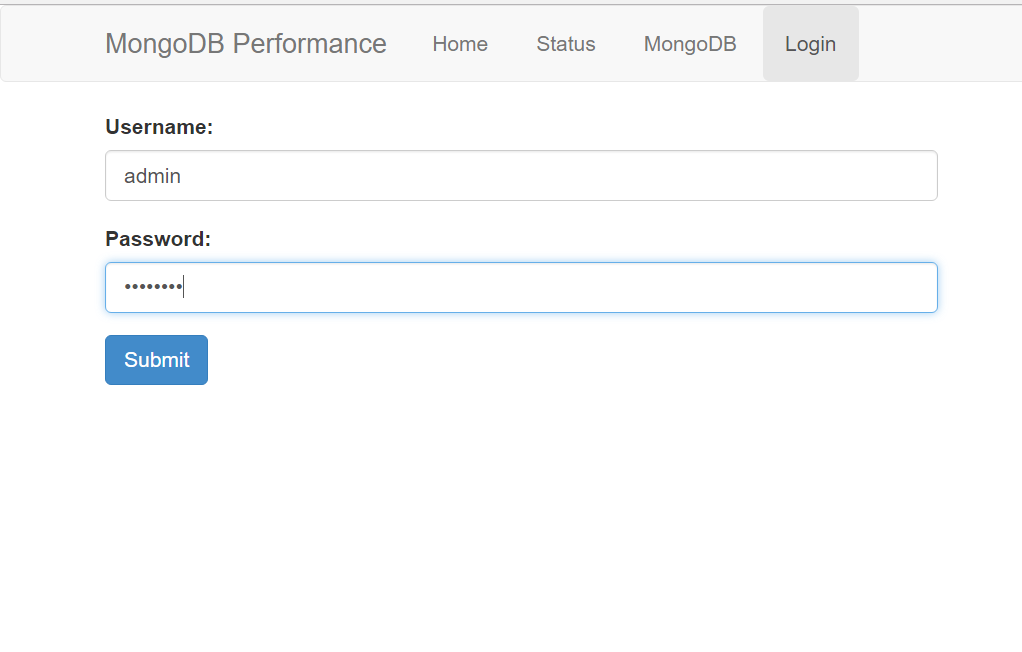
\includegraphics[scale=0.5]{login.png}
\centering
\caption{The Login page.}
\end{figure}
The \textit{Home Page} simply introduce the user to the application with a welcoming message.
The \textit{Status Page} is  a page that launches a REST \footnote{https://en.wikipedia.org/wiki/Representational\_state\_transfer} call to all modules that are supposed to be in the application to check and monitor their status, then it prompts the result on screen. It makes easy to discover if a module, even running on another machine, is not answering allowing the user to quickly resolve the problem.
\begin{figure}[H]
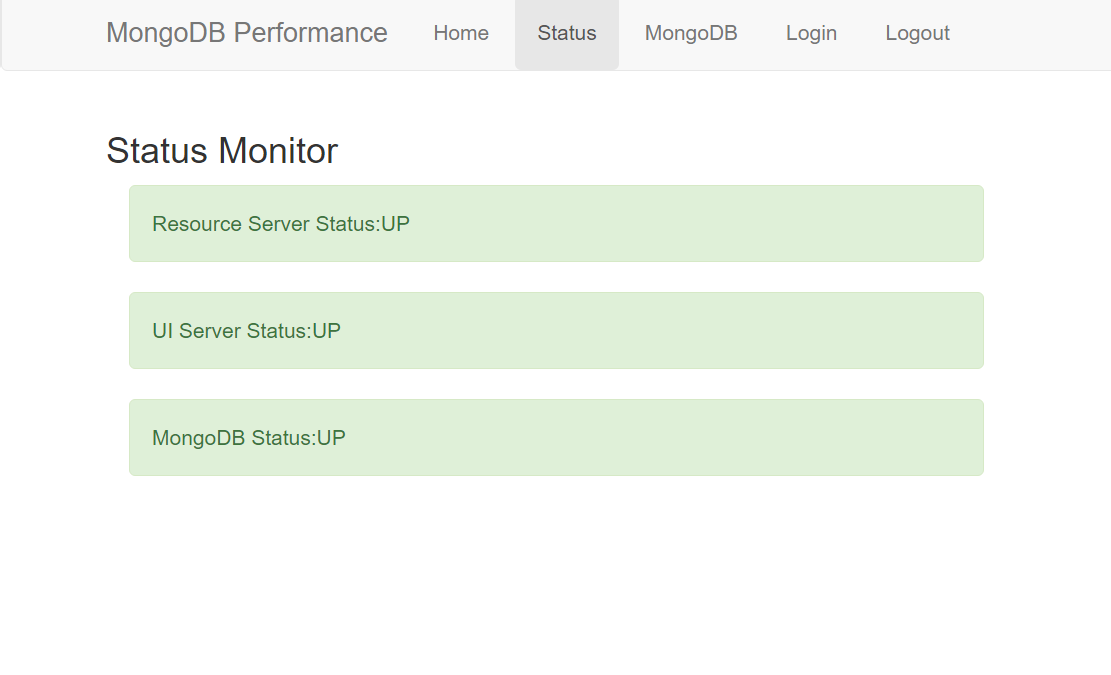
\includegraphics[scale=0.5]{status.png}
\centering
\caption{The Status page.}
\end{figure}
The\textit{MongoDB Page} is the most important of this module and  it is the page where the user can set up the configuration for a new test.
It is possible to choose:
\begin{itemize}
	\item The\textit{ number of entries} or inserts that has to be performed during the whole test
	\item The \textit{number of threads}, each one simulates a new client connecting to the MongoDB node. It is important to specify that the number of entries of each thread will be the total number of entries / the total number of threads. There is no real limit to the number that can be set, but a normal notebook will begin to suffer with more than 8 threads as the Java Virtual Machine is pretty expensive on the CPU and on the RAM. We will see further the specifications of the machines used during the experiment and how many threads have been used for the test.
	\item The \textit{type of test}, using only \textsc{put} statements (only inserts), only \textsc{get} statements (only gets, never used in practice) or \textsc{put/get} statements (one insert and then one get for each entry).
	\item The \textit{IP address} of the machine or computer running an instance of the Resource Module, to choose where start a test or to monitor an already running test on a specific machine.
\end{itemize}
\begin{figure}[H]
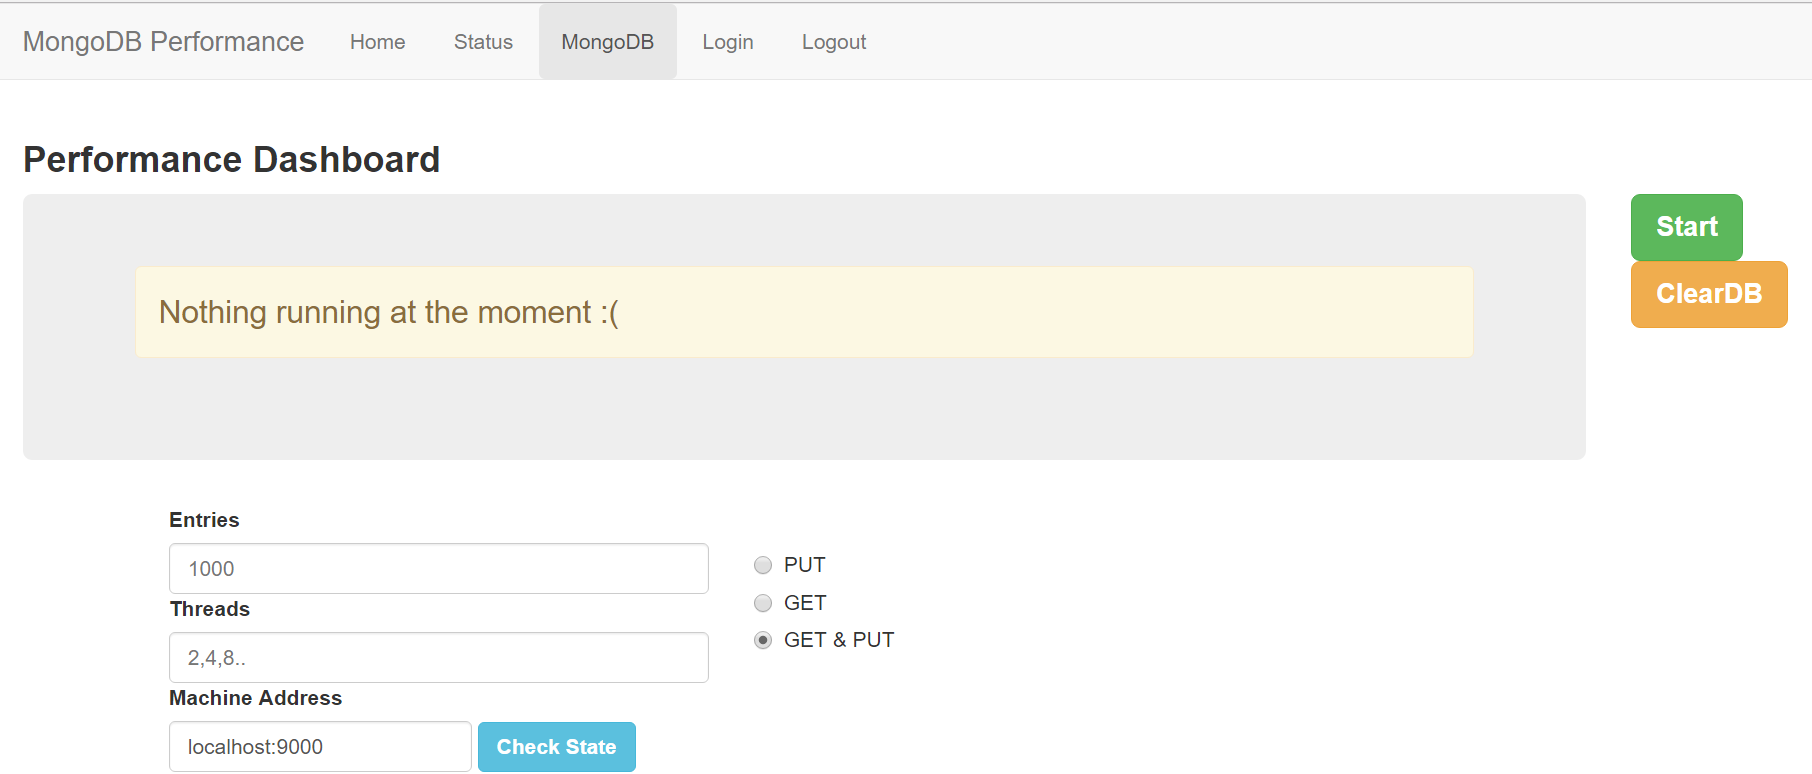
\includegraphics[scale=0.3]{test-off.png}
\centering
\caption{The MongoDB page.}
\end{figure}
It is  possible to drop all the records in the database to clean it up before a new test using the button “ClearDB”. When everything is set up, or using default values, it is possible to “Launch” the test and open  new view that shows any possible information about the running test. It is important to specify that in absence of a responding Resource Module, the test won’t start because all the metrics are calculated in that module and fetched through REST calls.
If everything is correctly set up, the test will start and all metrics calculated on Mongo are fetched and showed in the top table.
\begin{figure}[H]
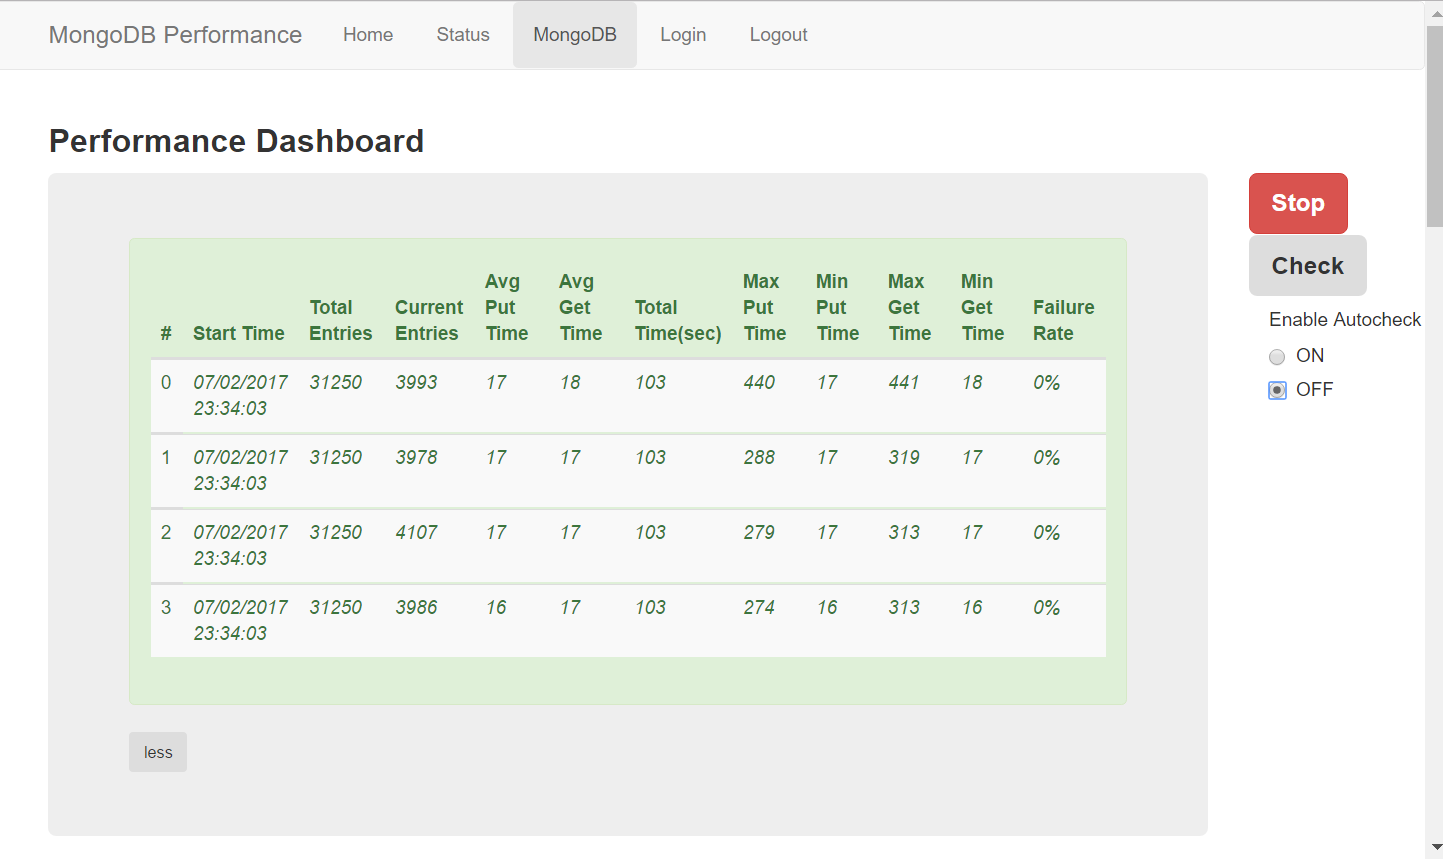
\includegraphics[scale=0.4]{metriche.png}
\centering
\caption{Table of the metrics.}
\end{figure}
It is possible to plot  the most interesting metrics in real time with “AutoDraw”  , but this option is disabled by default due to the heavy cost in terms of memory for the computer. It is anyway possible to plot metrics at the end of the test with “Draw” because all data are saved in variables until the test is not stopped. All graphs and tables that will be presented in the tests have been plotted by the application and saved at the end of each test.
\begin{figure}[H]
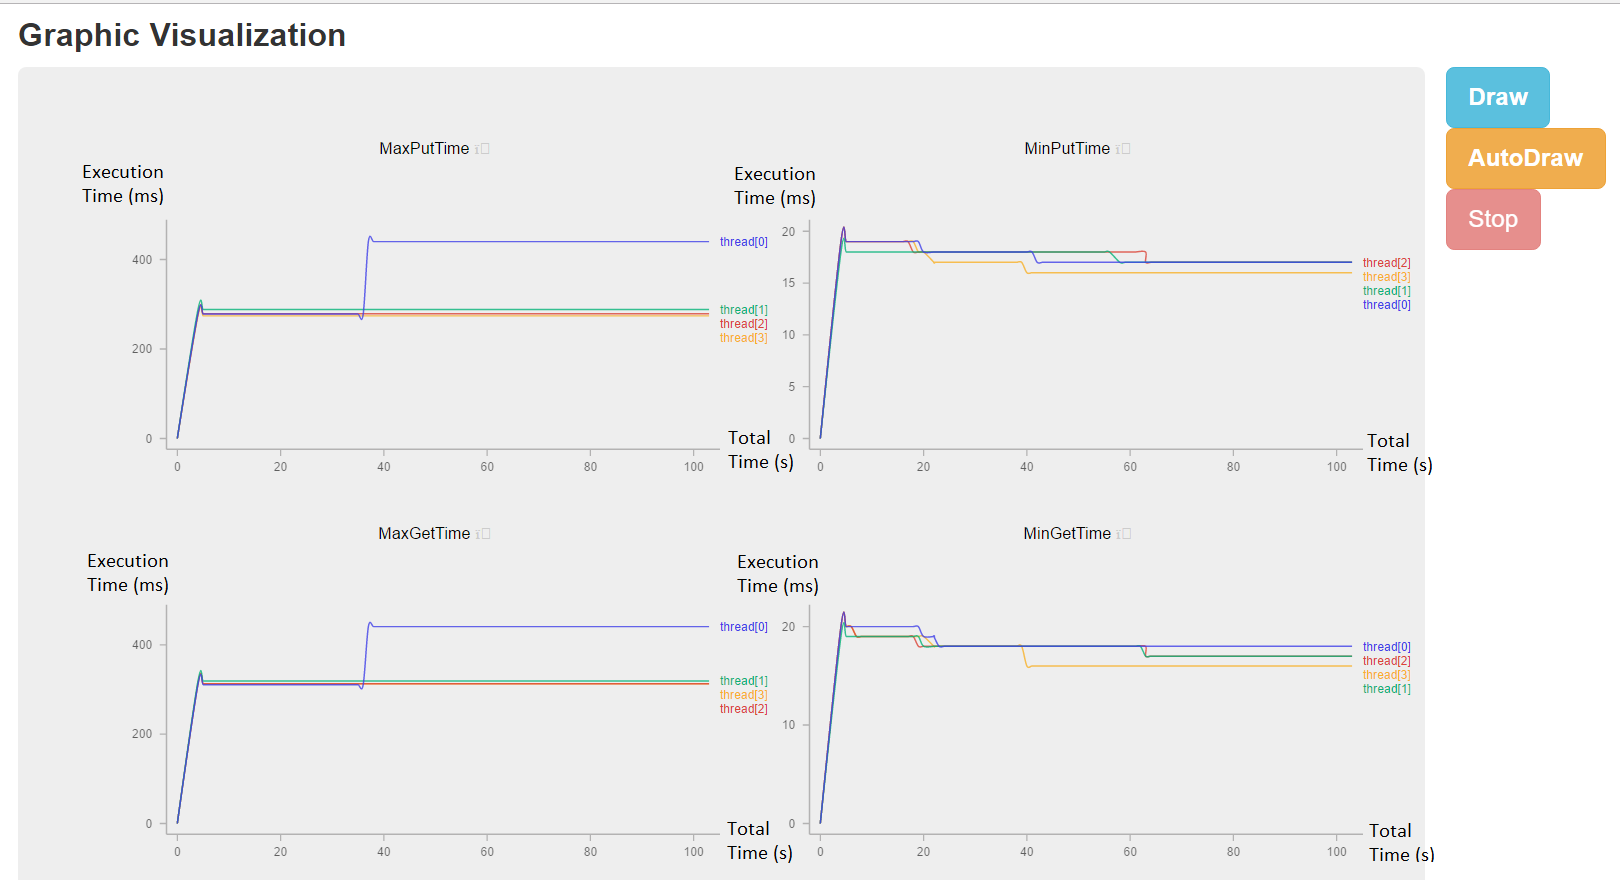
\includegraphics[scale=0.6]{grafici_corretti.png}
\centering
\caption{Graphics of Min/Max Put/Get times.}
\end{figure}
\begin{figure}[H]
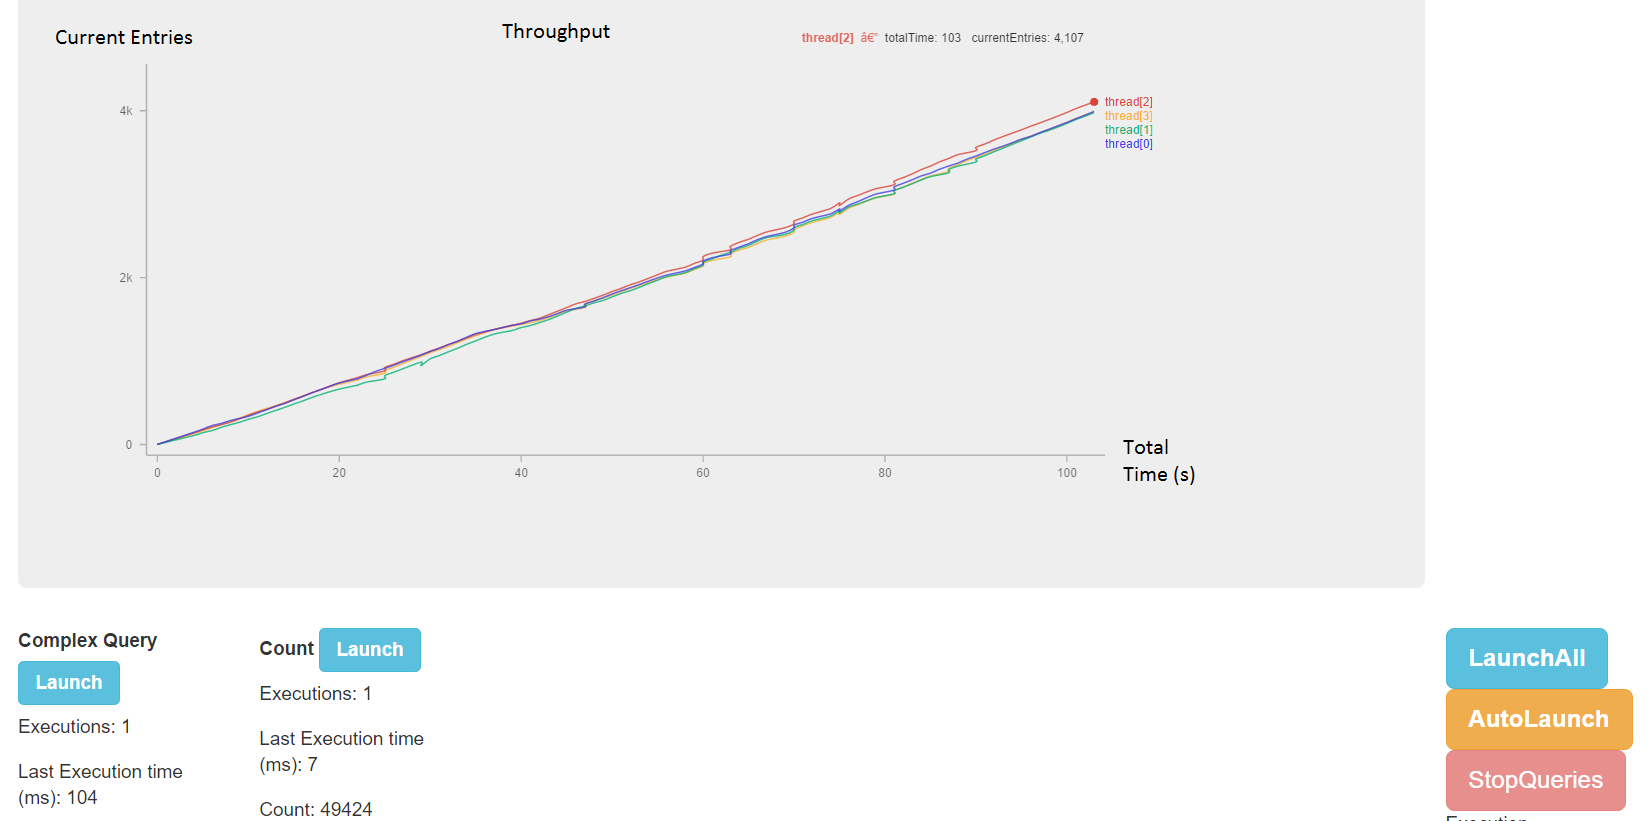
\includegraphics[scale=0.5]{queries_corrette.png}
\centering
\caption{Graphic of Throughput and query commands.}
\end{figure}
At the bottom of the page there are two buttons that can launch specific queries:
\begin{itemize}
	\item \textit{countAll( )} - Query that returns all the current records in the database. The main reason for this was to double check the insertions and see if they matched the values printed in the metrics table.
	\item \textit{complexQuery( )} - Query with the purpose to stress the  process of insert and get of the entries, it was used in specific tests with heavy workload and its times of execution where saved and then plotted in a secondary moment. When launched in “Auto” it runs every 10 seconds and updates an array containing all the execution times that will be plotted.\footnote{See section 4.4}
\end{itemize}



\subsection{MongoDB Resource module}
This is the core module of the application. All endpoints for the REST calls from the UI Module are defined and connected to a specific function in this module. It is not necessary to have an UI Module to run a test since it is possible to launch the standalone .jar of the Resource Module from command line and setup a test following the options printed on screen. It is possible to print some metrics on the console, but this functionality has never been used during the benchmark due to the necessity of plotting data on the UI.
\begin{figure}[H]
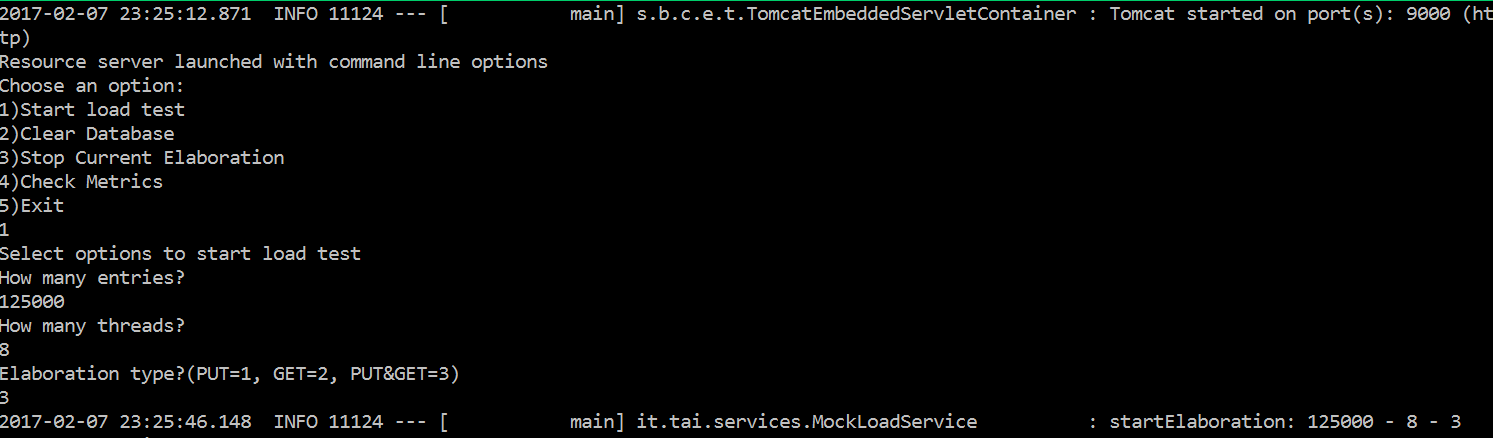
\includegraphics[scale=0.4]{command-line.png}
\centering
\caption{The Resource Module in the Linux shell.}
\end{figure}
It is possible to connect the UI Module to different instances of the Resource Modules even running of different machines to fetch all possible data, and this is how the tests have been conducted.
In this module is also defined the structure of \textit{Fattura.java}, the type of document used for the tests, and the repository that connects to the MongoDB collection Test where the data are stored. The core class of the module is \textit{MockLoadService.java} where resides the algorithm that process the benchmark and where all the metrics are calculated and saved.
The algorithm takes as parameters the number of entries, the type of test and most important the number of threads; then for each thread it replicates the process simulating a new client connection on the database.

      \newpage
      \chapter{Tests and results}
\label{cha:4}
In this last chapter we discuss the results of the tests, focusing on some particular metrics in relation to the specifications given at the beginning of the project. For the environment of testing we created a small network of virtual machines that could properly stress testing a Mongo database and give a more realistic feedback in terms of network overhead.
Proceeding through the chapter, we deeply explain each metric analyzed and compare the results between different test cases.

\section{Environment of testing}
\label{sec:1}
Since multithreading inside the Java Virtual Machine is quite expensive in terms of CPU and memory usage, it was not possible to launch more than 8 threads from a single machine. 
The environment of testing is a small LAN of virtual and physical machines connected and controlled in SSH \footnote{http://www.cisco.com/c/en/us/about/press/internet-protocol-journal/back-issues/table-contents-46/124-ssh.html} using Putty from a laptop.
The following virtual machines are part of the evironment: 
\begin{itemize}
	\item \textit{vm-mondb} running a Mongo node as Master with the following hardware specifications - CPU: Intel i7 Quadcore @2400Mhz, RAM: 4Gb, HDD: 30Gb.
	\item \textit{vm-mondb2} running a Mongo secondary node as Slave with the following hardware specifications - CPU: Intel i7 Quadcore @2400Mhz, RAM: 4Gb, HDD: 30Gb.
	\item \textit{vm01-st} and \textit{vm02-st} running the MongoDB Resource standalone module with the following specifications - CPU: QEMU Quadcore @1800Mhz, RAM: 4Gb, HDD: 6,7Gb.
	\item \textit{vm03-st} running the MongoDB Resource standalone module with the following specifications - CPU: QEMU Dualcore @1800Mhz, RAM: 4Gb, HDD: 5,3Gb.
\end{itemize}
\begin{figure}[H]
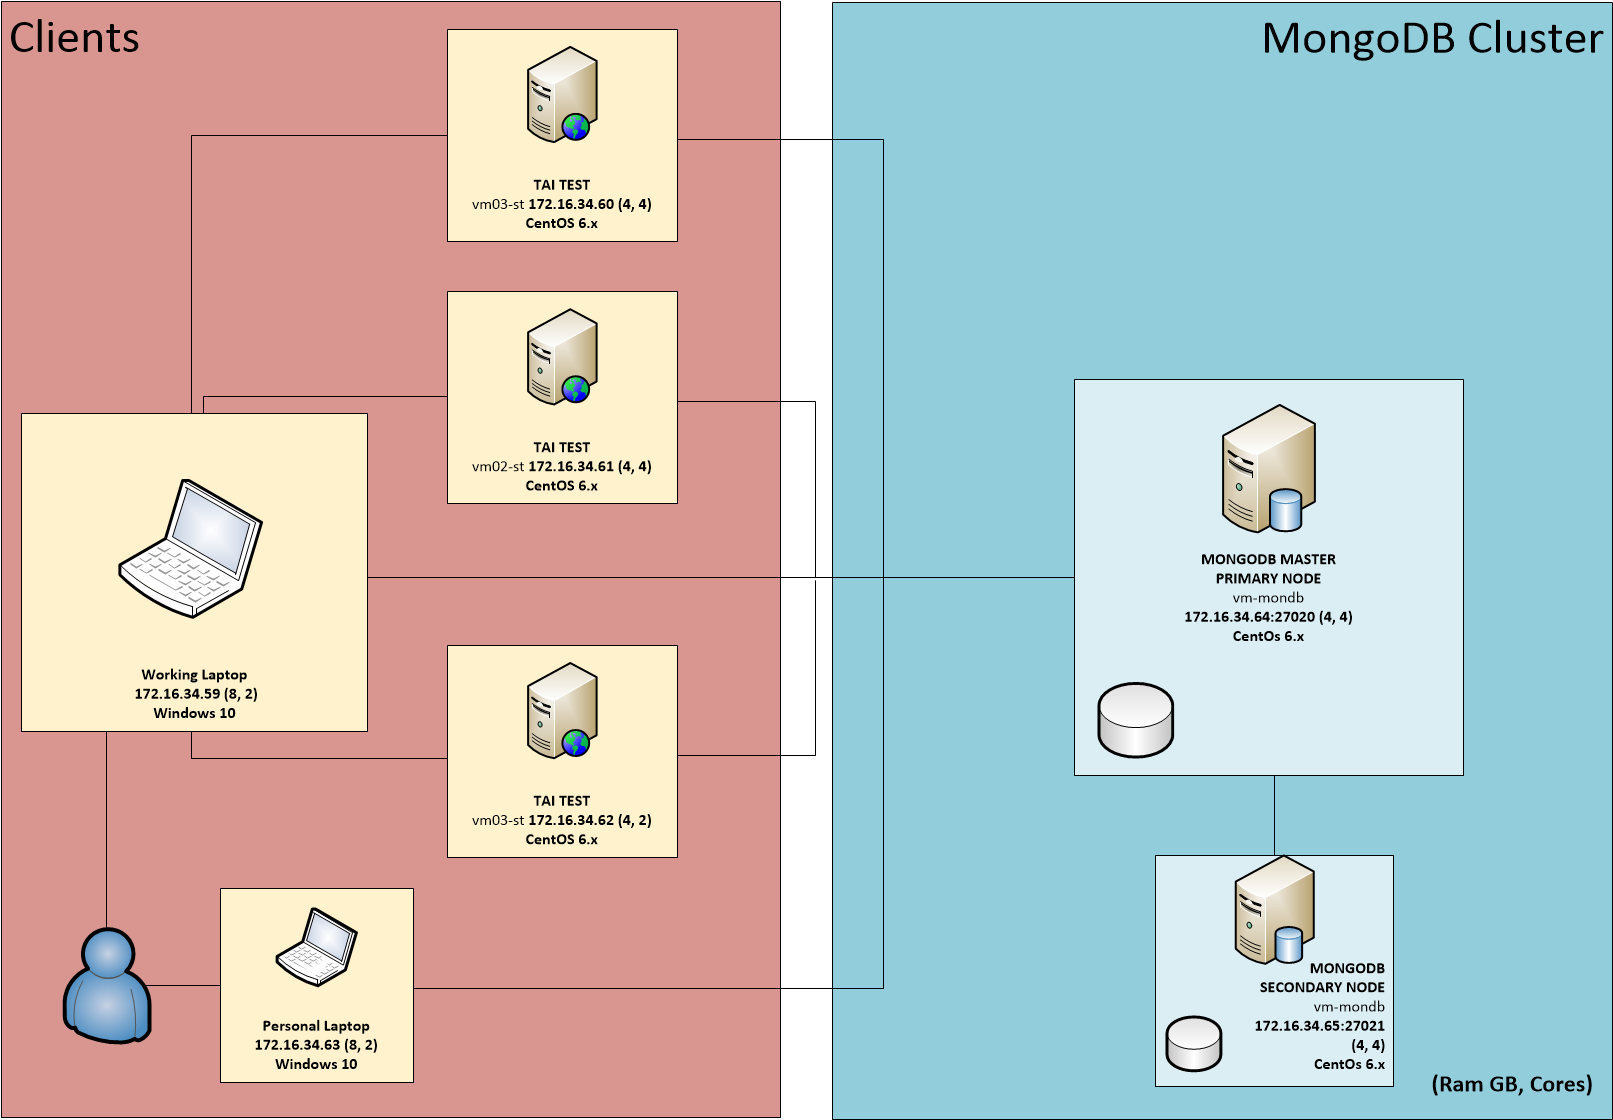
\includegraphics[scale=0.5]{my_architecture.png}
\centering
\caption{Representation of the environment of testing.}
\end{figure}
Every virtual machine was running a Linux distribution, CentOS, and they were controlled simultaneously using Putty. On every  client machine an instance of the MongoDB Resource Module was running from the Linux shell with same test configuration.
On the machines hosting the Mongo nodes, Mongo had two different configurations: 


The primary node was running a \textit{mongod} \footnote{See section 2.5} instance with 2 different \textit{config servers} \footnote{See section 2.6}. This configuration allowed to quickly switch from a single- node configuration to a double-node (or more) configuration.
\begin{lstlisting}
# mongod.conf

# for documentation of all options, see:
#   http://docs.mongodb.org/manual/reference/configuration-options/

# where to write logging data.
systemLog:
  destination: file
  logAppend: true
  path: /var/log/mongodb/mongod_configsvr.log

# Where and how to store data.
storage:
  dbPath: /var/lib/mongo
  journal:
    enabled: true
#  engine:
#  mmapv1:
#  wiredTiger:

# how the process runs
processManagement:
  fork: true  # fork and run in background
  pidFilePath: /var/run/mongodb/mongod_configsvr.pid  # location of pidfile
  #pidFilePath: /var/run/mongodb/mongod_configsvr2.pid # location of pidfile for 2 nodes configuration

# network interfaces
net:
  port: 27021
#  bindIp: 127.0.0.1  # Listen to local interface only, comment to listen on all interfaces.

#security:

#operationProfiling:

#replication:

#sharding:

## Enterprise-Only Options

#auditLog:

#snmp:
\end{lstlisting}

\newpage
The secondary node was running a \textit{mongos} instance instead, that automatically connects to the primary node in case the configuration for 2 nodes is set. \textit{Replica Set} was not enabled because in a benchmark test it would only affect performance and it is usually a production choice where it could provide consistency and durability of the data.

\begin{lstlisting}
# mongos.conf

# for documentation of all options, see:
#   http://docs.mongodb.org/manual/reference/configuration-options/

# where to write logging data.
systemLog:
  destination: file
  logAppend: true
  path: /var/log/mongodb/mongos.log

# Where and how to store data.
#storage:
#  dbPath: /var/lib/mongo
#  journal:
#    enabled: true
#  engine:
#  mmapv1:
#  wiredTiger:

# how the process runs
processManagement:
  fork: true  # fork and run in background
  pidFilePath: /var/run/mongodb/mongos.pid  # location of pidfile

# network interfaces
net:
  port: 27020
#  bindIp: 127.0.0.1  # Listen to local interface only, comment to listen on all interfaces.


#security:

#operationProfiling:

#replication:

sharding:
  configDB: vm-mondb:27020

## Enterprise-Only Options

#auditLog:

#snmp:
\end{lstlisting}

 
\section{Test cases and setup}
\label{sec:2}
Basically, three different tests have run with both configurations of Mongo (with one and with two nodes). 
The plan was to perform tests of increasing complexity and data workload to analyze the differences between their results and to  understand how Mongo reacts under stressing conditions.
\begin{itemize}
	\item \textit{First Type} : this type tests every main feature of the software and  give a first overview on Mongo performance in normal conditions.
	\item \textit{Second Type} : this type heavily stresses Mongo with multiple parallel connections and inserting at maximum speed 2.000.000 of documents. It was used to analyze Mongo scalability rate from 1 to 2 nodes.
	\item \textit{Third Type} : this type has the same stressing purpose as Second Type with identical configuration, in addition it executes a specific search using as parameter a random number assigned to each document. This query is executed every 10 seconds for 750 times returning an increasing set of matching documents.
\end{itemize}


\section{Gathering data}
\label{sec:3}
In this phase all data spread across 4 different instances of MongoDB Resource Module have been gathered using the UI Module on a laptop connected to the LAN.
In the meanwhile on another laptop the UI Module plotted all the data of its MongoDB Resource Module instance. It was not possible to plot the results from the virtual machines because their data did not pass through the Angular module dedicated to this function. This is unfortunately a limitation of the actual implementation of the software.
All the metrics tables and the graphs plotted by the UI module were printed on .jpeg files and then inserted into an Excel Spreadsheet where there is a page for each test. All the averages from all the machines for each test have been calculated using Excel inside the relative page and then linked to the summary page to compare all the tests. Any plotted graph has been linked into those pages but not into the summary page to allow a clean presentation to any reader.
This Excel Spreadsheet \footnote{https://drive.google.com/open?id=0B1IlD5PLfM8\_LTY5QjVXR0R3SE0} is freely available for consultation. 
It is possible to read all the data retrieved from the tests, but as they are quite a lot and eventually confusing, only the most interesting and meaningful are analyzed in the following sections. For more details, all readers are free to consult that file.

\section{Analyzing results}
\label{sec:4}

\subsection{Description of the metrics analyzed}
Before going deeper into the analysis, we are going to explain which metrics have been analyzed and how they have been calculated:
\begin{itemize}
	\item \textit{Average Put Time / Average Get Time} : respectively average time of insertion and retrieve of a document into/from the database.
	\item \textit{Max Put Time / Min Put Time} : respectively maximum and minimum time of insertion into the database.
	\item \textit{Max Get Time / Min Get Time} : respectively maximum and minimum time of insertion into the database.
	\item \textit{Throughput} : total amount of operations (put and get) divided by the total time needed to complete the workload of the test.
	\item \textit{Failure Rate} :total number of failed operations (that returned an exception) over the total number of operations performed.
\end{itemize}
There are some approximations in the metrics presented in the \textit{Summary page} of the Excel Spreadsheet due to the high number of running threads on different machines:
\begin{itemize}
	\item \textit{Test Duration} : it refers to the time taken by the slowest machine of each test to complete the workload. It is not the time used to calculate \textit{Throughput}.
	\item \textit{Avg Put/Get Times} : those are the average of the Average Put/Get Times calculated on each machine in a test.
	\item \textit{Max and Min Put/Get Times} : those are the maximum and the minimum put/get times overall of a test.
	\item \textit{Throughput} : it is the average the Throughput calculated on each machine in a test, so for example if a machine took time "T" to perform "n" operations on "i" machines, the formula to obtain this final throughput is: 
\[Throughput = \frac{\sum_{0}^{i}\frac{n_{i}}{T_{i}}}{i}\]

\end{itemize}
Now that we have defined the meaning of those values, we can analyze the most significant tests.
\subsection{Analyzed Tests}
A total number of 10 tests have been performed using \textsc{MongoDb Performance}, but some of them failed or were not relevant.
We take in account only \textit{Test1}, \textit{Test4}, \textit{Test6} and \textit{Test10} because for the following reasons the others cannot be relevant.
Tests from 1 to 3 are not real load tests, they did not “stress” Mongo at all, so only one of them is presented as example.
\textit{Test5} suffered the desynchronization of the OS time clock of a Mongo node with the other of about half an hour, and since Mongo assigns \textit{\_id} using timestamp of the machine and then balances documents between the nodes on a Shard Key that includes by default \textit{\_id} \footnote{This is a good reason to specify a Shard Key on a different field.}, the two nodes lost performance and data were divided approximately 60\% on the first node and 40\% on the second node. 
Each test  took some hours to run, some of them have scheduled for automatic launch during the night to save time.
For unknown reasons, \textit{Test7} and  \textit{Test9} were incomplete due to an interruption of alimentation of the laptop used to plot data \footnote{The laptop itself was running threads that unfortunately stopped performing operations on Mongo}.
As last, we can ignore \textit{Test8} as the complexity of the query used to stress Mongo was too low with to affect the database performance, resulting in a test similar to \textit{Test4}.
Anyway, all machines that completely performed their workload have been kept in the analysis because there was no time to repeat the tests before the presentation scheduled date and they still confirmed Mongo efficient performance \footnote{Data were partially comparable}.

\subsection{Results}
the table gathers the most relevant results from the analysis spreadsheet, cleaned from all unnecessary columns and details.
%\begin{figure}[H]
%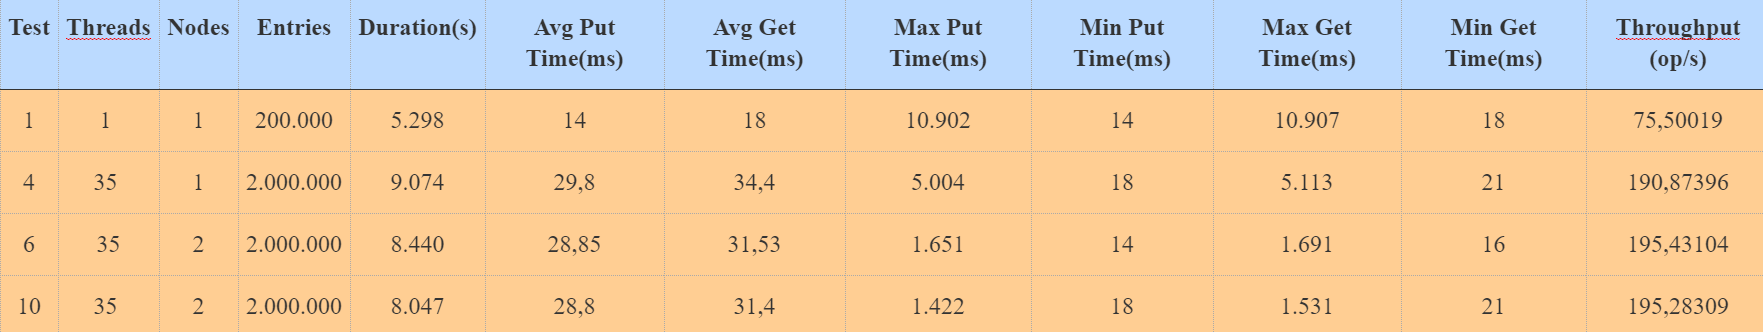
\includegraphics[scale=0.3]{table.png}
%\centering
%\caption{Summary of the analyzed metrics.}
%\end{figure}
\begin{table}[H]
\centering
\label{my-label}
\begin{tabular}{@{}ccccccc@{}}
\toprule
\rowcolor[HTML]{BBDAFF} 
Test & Threads & Nodes & Entries & Duration(s) & Avg Put Time(ms) & Avg Get Time(ms) \\ \midrule
\rowcolor[HTML]{FFCC67} 
1 & 1 & 1 & 200.000 & 5.298 & 14 & 18 \\
\rowcolor[HTML]{FFCC67} 
4 & 35 & 1 & 2.000.000 & 9.074 & 29,8 & 34,4 \\
\rowcolor[HTML]{FFCC67} 
6 & 35 & 2 & 2.000.000 & 8.440 & 28,85 & 31,53 \\
\rowcolor[HTML]{FFCC67} 
10 & 35 & 2 & 2.000.000 & 8.047 & 28,8 & 31,4 \\ \bottomrule
\end{tabular}
\end{table}

\begin{table}[H]
\centering
\begin{tabular}{@{}cccccc@{}}
\toprule
\rowcolor[HTML]{BBDAFF} 
Test & \begin{tabular}[c]{@{}c@{}}Max\\  Put Time(ms)\end{tabular} & \begin{tabular}[c]{@{}c@{}}Min\\ Put Time(ms)\end{tabular} & \begin{tabular}[c]{@{}c@{}}Max \\ Get Time(ms)\end{tabular} & \begin{tabular}[c]{@{}c@{}}Min \\ Get Time(ms)\end{tabular} & Throughput(op/s) \\ \midrule
\rowcolor[HTML]{FFCC67} 
1 & 10.902 & 14 & 10.907 & 18 & 75,50019 \\
\rowcolor[HTML]{FFCC67} 
4 & 5.004 & 18 & 5.113 & 21 & 190,87396 \\
\rowcolor[HTML]{FFCC67} 
6 & 1.651 & 14 & 1.691 & 16 & 195,43104 \\
\rowcolor[HTML]{FFCC67} 
10 & 1.422 & 18 & 1.531 & 21 & 195,28309 \\ \bottomrule
\end{tabular}
\caption{Summary of the analyzed metrics.}
\label{my-label}
\end{table}

All of those tests run with a 50 – 50 workload type, meaning that half of the operation were \textit{put} operations and the other half \textit{get} operations, for example having 200.000 entries means that 400.000 operations are performed during the test.
There are three different typologies of test \footnote{See section 4.2} so we analyze at least one test for each typology: Test 1 belongs to the First Type and so it was just a functional test with a small workload performed on a Mongo database with 1 node. It obtained a \textit{Max Put Time} and a \textit{Max Get Time} of more than 10 seconds, but some considerations should be taken in account:
\begin{itemize}
	\item Each \textit{get} operation happen after a \textit{put} operation, so it’s reasonable to assume that \textit{Max Get Time} of 10.907 ms is  the result of \textit{Max Put Time} + 5 ms \footnote{In simple words, get time is anyway acceptable.}.
	\item \textit{Avg Put Time} and \textit{Avg Get Time} stay on really low values, respectively 14 ms and 18 ms, that in first place satisfies the customer requisite of 2 seconds to retrieve data from the database. In second place it means that since they are average values and they do not appear to be affected by \textit{Max Put/Get Time},  those “worse" cases are just a very few over the total operations performed.
\end{itemize}
\textit{Test 4} and \textit{Test 6} belong to the Second Type, they are stress tests performed with same configuration. In total they execute 2 million entries \footnote {4.000.000 operations with this type of workload} running 35 parallel threads with all virtual machines available. The only difference between them is that \textit{Test 4} runs on a Mongo database with 1 node while \textit{Test 6} runs on a Mongo database with 2 nodes and a Shard Key on the \textit{\_id} field.
It is possible to appreciate how Mongo scales well horizontally by adding nodes to its configuration. First, \textit{Duration} is a bit shorter and \textit{Avg Put/Get Times} are slightly better. Most important is that with multiple nodes none of the operations took more than 1,7 seconds to execute. This means that Mongo manages concurrency more efficiently with more nodes, that is what we expected in terms of scalability and distribution of data. In the average, Mongo performed 5 more operations each second using 2 nodes.
At last, \textit{Test 10} belongs to Third Type and was performed with the same configuration as \textit{Test 6} \footnote{35 threads, 2 millions entries, 2 nodes}, but with an additional single field index on the field \textit{rIndex}, containing a random generated number between 0 and 3.000.000.
During this test along with other operations, a "Complex Query" have been automatically executed every 10 seconds for a total of 750 times on the database. This query takes a random number  R between 0 and 2.999.900 and retrieves all the documents having  \textit{rIndex} in the set \{R , R+100\}.
With the progressive increase of \textit{n} as total number of documents in the database, the query takes increasing average time to execute. 
The following chart represents all execution times of the query over the total executions.
\begin{figure}[H]
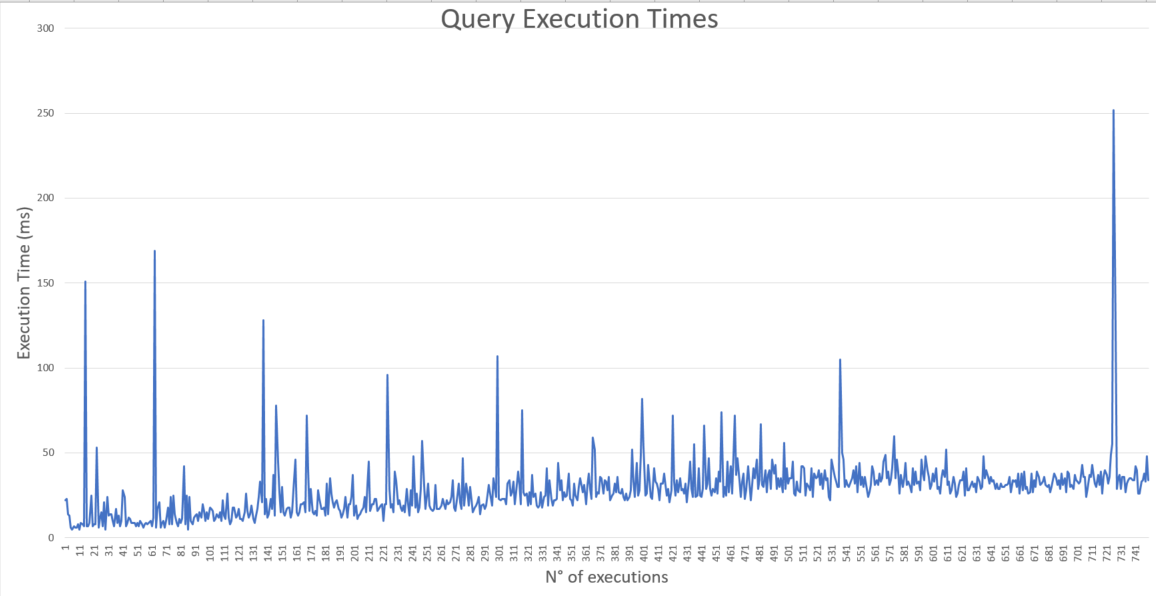
\includegraphics[scale=0.55]{exec_times_new.png}
\centering
\caption{Query execution times.}
\end{figure}
The average time of execution appears to increase following a logarithmic curve and this is consistent with MongoDB implementation of data structures research .
In fact, Mongo uses B+ Trees as data structure and consequently the complexity of a \textit{find( )} function is O(logn).
This great result obviously has a cost: \textit{Min Put/Get Times} have a worse performance in our benchmark  because of the secondary index on \textit{rIndex}. 
Even if  there are not evident differences in the \textit{Avg Put/Get Times}, the \textit{Throughput} slightly decreases and probably with a higher number of documents it would become more perceptible.
In a production software anyway there are usually less insert operations than get operations, therefore using indexes with a small cost on the insertion time is completely worth the increase of reading speed.
In conclusion, low average times to perform query data, no data loss \footnote{0\% failure rate in every test } and an appreciable scalability even using  “weak” hardware specifications, MongoDB confirms to be a choice that perfectly fits the needs of our commission.
\section{Comparing results with other benchmarks}
\label{sec:5}
In the spreadsheet summary, there are also some results of tests performed by other two companies with better hardware components to support bigger workloads. Those benchmarks have been used in the beginning of the project as inspiration and also as first overview on Mongo and its performance with a proper hardware.
Unfortunately they cannot be compared with our results in the end.
The main problem with many benchmarks available on the web is that they are often committed, or even performed, by companies that own a NoSQL solution to show its streght over the others.
This lead to a problem of advertising part and to specific benchmark tests made within ad-hoc situations in which a certain NoSQL database performs at its best.
Anyway, most of the benchmarks agree that the NoSQL database that actually gains most from Horizontal Scalability is Apache Cassandra thanks to its Key-Value implementation.
Other NoSQL solutions are better in some particular use cases, consequently when a company decides to migrate to a new NoSQL solutions  it should try to find the one that fit its specific needs.

      \newpage
      \chapter{Conclusion}
\label{cha:conclusion}
After this evaluation and the presentation of the results, Mongo was confirmed for the new commission. In particular, some considerations had a great impact on the decision: Mongo's ability to support and scan a huge number of records under stress, the low average time needed to retrieve data , the optimal failure rate of 0\% in every test and the simplicity of usage.
There are other NoSQL solutions that state better results in benchmarks, anyway Mongo gave us a sensation of strenght and soundess without saving on performance.
For the future commission the storage architecture will possibily be supported by an SQL solution to store sensible data of the users of the application, while Mongo will be used as storage for all documents related to each user that will be in the grade of billions in the production deployment.
We can now summarize this research and point out some considerations focusing on this question: “how and where NoSQL databases are getting over Relational databases?”.
Looking at NoSQL brief history it seems clear that this technology was born as niche product developed by big IT companiest to support their needs. We can find a huge number of NoSQL databases on the internet all deriving their concepts and implementations from the very first and most famous of them: Amazon Dynamo, Apache Cassandra, Google Big Table and MongoDB.
In the very following years after the concept of NoSQL was born, pretty much every IT company working with Big Data was developing its own version from those models, following specific “needs” but also “fashion”.
SQL and RDBMS will not disappear as they have been a standard for over 30 years and in many use cases where the amount of data is in the grade of Gigabytes, RDBMS  have good performance sometimes even better than many NoSQL databases and will always guarantee ACID propertis that are fundamental in many use cases
It is important to underline that a developer expert of SQL will be an expert user of any kind of RDBMS, while a developer with experience on MongoDB will probably need to learn Apache Cassandra from the very beginning because there is no real standard in NoSQL, each one of them have a proprietary implementation.
But over this consideration and over the performance consideratio, NoSQL technologies have some advantages that will always grant them a step over Relational databases:
\begin{itemize}
	\item Most of them have an open source edition maintained by their companies.
	\item Any developer of the most used programming language such as C++, Java, Python, Perl, C\#, etc. will have no real problem to learn and interface with a NoSQL database.
	\item Most of them are easy to scale and easy to maintain, with consequent saving on time and costs.
	\item They are the only who can support Big Data, a reality of the market that cannot be ignored.
\end{itemize}
Because of those reasons, now NoSQL databases are relegating Relational Databases to more niche roles and getting over as common choice for a storage technology.
In my personal considerations, SQL and NoSQL technologies will keep working in parallel for long time as Specialization is what makes each part of a system obtain the best result for the system itself, and some choices are better than others in specific roles.
Many computer scientists have already started conceiving the concept of \textit{NewSQL} \cite{corbellini}, and some databases have already emerged under the name of “NewSQL databases”, for example NuoDB, VoltDB and Clustrix.
In fact, those databases are actually Relational databases supporting automatic replication, sharding and distributed transactions, i.e. providing ACID guarantees even across shards. 
It is hard to establish what will be the future of storage technologies but in the following years any kind of Databases-related course should be ready to teach students a new way of thinking how to design a database among the classic concepts inherited from the Relational Model.
In this way, next generation of developers will be ready for the new challenge  that NoSQL technologies have opened to our world in terms of storing, manipulating and retrieving data to support the increasing amount of information exchanged through the Web.


      \newpage
      
      
    \endgroup


    % bibliografia in formato bibtex
    %
    % aggiunta del capitolo nell'indice
    \addcontentsline{toc}{chapter}{Bibliografia}
    % stile con ordinamento alfabetico in funzione degli autori
    \bibliographystyle{plain}
    \bibliography{biblio}
%%%%%%%%%%%%%%%%%%%%%%%%%%%%%%%%%%%%%%%%%%%%%%%%%%%%%%%%%%%%%%%%%%%%%%%%%%
%%%%%%%%%%%%%%%%%%%%%%%%%%%%%%%%%%%%%%%%%%%%%%%%%%%%%%%%%%%%%%%%%%%%%%%%%%
%% Nota
%%%%%%%%%%%%%%%%%%%%%%%%%%%%%%%%%%%%%%%%%%%%%%%%%%%%%%%%%%%%%%%%%%%%%%%%%%
%% Nella bibliografia devono essere riportati tutte le fonti consultate 
%% per lo svolgimento della tesi. La bibliografia deve essere redatta 
%% in ordine alfabetico sul cognome del primo autore. 
%% 
%% La forma della citazione bibliografica va inserita secondo la fonte utilizzata:
%% 
%% LIBRI
%% Cognome e iniziale del nome autore/autori, la data di edizione, titolo, casa editrice, eventuale numero dell’edizione. 
%% 
%% ARTICOLI DI RIVISTA
%% Cognome e iniziale del nome autore/autori, titolo articolo, titolo rivista, volume, numero, numero di pagine.
%% 
%% ARTICOLI DI CONFERENZA
%% Cognome e iniziale del nome autore/autori (anno), titolo articolo, titolo conferenza, luogo della conferenza (città e paese), date della conferenza, numero di pagine. 
%% 
%% SITOGRAFIA
%% La sitografia contiene un elenco di indirizzi Web consultati e disposti in ordine alfabetico. 
%% E’ necessario:
%%   Copiare la URL (l’indirizzo web) specifica della pagina consultata
%%   Se disponibile, indicare il cognome e nome dell’autore, il titolo ed eventuale sottotitolo del testo
%%   Se disponibile, inserire la data di ultima consultazione della risorsa (gg/mm/aaaa).    
%%%%%%%%%%%%%%%%%%%%%%%%%%%%%%%%%%%%%%%%%%%%%%%%%%%%%%%%%%%%%%%%%%%%%%%%%%
%%%%%%%%%%%%%%%%%%%%%%%%%%%%%%%%%%%%%%%%%%%%%%%%%%%%%%%%%%%%%%%%%%%%%%%%%%
    

    \titleformat{\chapter}
        {\normalfont\Huge\bfseries}{Allegato \thechapter}{1em}{}
    % sezione Allegati - opzionale
    \appendix
   % \chapter{Titolo primo allegato}

Lorem ipsum dolor sit amet, consectetur adipiscing elit. Donec sed nunc orci. Aliquam nec nisl vitae sapien pulvinar dictum quis non urna. Suspendisse at dui a erat aliquam vestibulum. Quisque ultrices pellentesque pellentesque. Pellentesque egestas quam sed blandit tempus. Sed congue nec risus posuere euismod. Maecenas ut lacus id mauris sagittis egestas a eu dui. Class aptent taciti sociosqu ad litora torquent per conubia nostra, per inceptos himenaeos. Pellentesque at ultrices tellus. Ut eu purus eget sem iaculis ultricies sed non lorem. Curabitur gravida dui eget ex vestibulum venenatis. Phasellus gravida tellus velit, non eleifend justo lobortis eget. 

\section{Titolo}
Lorem ipsum dolor sit amet, consectetur adipiscing elit. Donec sed nunc orci. Aliquam nec nisl vitae sapien pulvinar dictum quis non urna. Suspendisse at dui a erat aliquam vestibulum. Quisque ultrices pellentesque pellentesque. Pellentesque egestas quam sed blandit tempus. Sed congue nec risus posuere euismod. Maecenas ut lacus id mauris sagittis egestas a eu dui. Class aptent taciti sociosqu ad litora torquent per conubia nostra, per inceptos himenaeos. Pellentesque at ultrices tellus. Ut eu purus eget sem iaculis ultricies sed non lorem. Curabitur gravida dui eget ex vestibulum venenatis. Phasellus gravida tellus velit, non eleifend justo lobortis eget. 

\subsection{Sottotitolo}
Lorem ipsum dolor sit amet, consectetur adipiscing elit. Donec sed nunc orci. Aliquam nec nisl vitae sapien pulvinar dictum quis non urna. Suspendisse at dui a erat aliquam vestibulum. Quisque ultrices pellentesque pellentesque. Pellentesque egestas quam sed blandit tempus. Sed congue nec risus posuere euismod. Maecenas ut lacus id mauris sagittis egestas a eu dui. Class aptent taciti sociosqu ad litora torquent per conubia nostra, per inceptos himenaeos. Pellentesque at ultrices tellus. Ut eu purus eget sem iaculis ultricies sed non lorem. Curabitur gravida dui eget ex vestibulum venenatis. Phasellus gravida tellus velit, non eleifend justo lobortis eget. 


\chapter{Titolo secondo allegato}

Lorem ipsum dolor sit amet, consectetur adipiscing elit. Donec sed nunc orci. Aliquam nec nisl vitae sapien pulvinar dictum quis non urna. Suspendisse at dui a erat aliquam vestibulum. Quisque ultrices pellentesque pellentesque. Pellentesque egestas quam sed blandit tempus. Sed congue nec risus posuere euismod. Maecenas ut lacus id mauris sagittis egestas a eu dui. Class aptent taciti sociosqu ad litora torquent per conubia nostra, per inceptos himenaeos. Pellentesque at ultrices tellus. Ut eu purus eget sem iaculis ultricies sed non lorem. Curabitur gravida dui eget ex vestibulum venenatis. Phasellus gravida tellus velit, non eleifend justo lobortis eget. 

\section{Titolo}
Lorem ipsum dolor sit amet, consectetur adipiscing elit. Donec sed nunc orci. Aliquam nec nisl vitae sapien pulvinar dictum quis non urna. Suspendisse at dui a erat aliquam vestibulum. Quisque ultrices pellentesque pellentesque. Pellentesque egestas quam sed blandit tempus. Sed congue nec risus posuere euismod. Maecenas ut lacus id mauris sagittis egestas a eu dui. Class aptent taciti sociosqu ad litora torquent per conubia nostra, per inceptos himenaeos. Pellentesque at ultrices tellus. Ut eu purus eget sem iaculis ultricies sed non lorem. Curabitur gravida dui eget ex vestibulum venenatis. Phasellus gravida tellus velit, non eleifend justo lobortis eget. 

\subsection{Sottotitolo}
Lorem ipsum dolor sit amet, consectetur adipiscing elit. Donec sed nunc orci. Aliquam nec nisl vitae sapien pulvinar dictum quis non urna. Suspendisse at dui a erat aliquam vestibulum. Quisque ultrices pellentesque pellentesque. Pellentesque egestas quam sed blandit tempus. Sed congue nec risus posuere euismod. Maecenas ut lacus id mauris sagittis egestas a eu dui. Class aptent taciti sociosqu ad litora torquent per conubia nostra, per inceptos himenaeos. Pellentesque at ultrices tellus. Ut eu purus eget sem iaculis ultricies sed non lorem. Curabitur gravida dui eget ex vestibulum venenatis. Phasellus gravida tellus velit, non eleifend justo lobortis eget. 




\end{document}
